\section{Feinentwurf}
Im folgenden Kapitel erhalten Sie eine Übersicht über die auf dem Client und dem Server verwendeten Klassen, welche die GoApp umsetzen sollen.\\

Um eine bessere Vorstellung davon zu bekommen, was unter sich immer wiederholenden Variablen verstanden wird, möchte ich diese an dieser Stelle vorstellen und erklären:\\

\begin{enumerate}
	\item GroupId: Eine GroupId ist eine neunstellige Integerzahl, welche mit einer 1 beginnt. Jede GroupId existiert genau einmal und macht es möglich, Gruppen eindeutig zu identifizieren.
	\item UserId: Eine UserId ist wie die GruppenId eine neunstellige Integerzahl, welche nicht mit einer 1 beginnt. Jede UserId existiert genau einmal und macht es möglich, Benutzer eindeutig zu identifizieren.
	\item GroupName: Ein Gruppenname kann bis zu 30 Zeichen lang sein und aus Groß- und Kleinbuchstaben bestehen und Sonderzeichen beinhalten. Jeder Gruppennanme muss eindeutig sein.
	\item UserName: Ein Benutzername kann wie der Gruppenname bis zu 30 Zeichen lang sein und aus Groß- und Kleinbuchstaben bestehen. Im Gegensatz zur Gruppe muss dieser Name nicht eindeutig sein.
	\item date: Das Datum eines Treffpunktes wird in dem Format dd.MM.yyyy dargstellt.
	\item time: Die Uhrzeit eines Treffpunktes wird in dem Format MM:HH dargestellt.
\end{enumerate}

\subsection{Clientseitig}
\subsubsection{ClientView}
\begin{enumerate}
	%- hier muss das PDF mit der Gesamtübersicht hin
	\item \textbf{\underline{MainActivity}}
	
	%- hier muss das PDF classcom_1_1example_1_1androidgoapp_1_1androidgoapp_1_1view_1_1_main_activity__inherit__graph.pdf eingebunden werden
	Aufgrund der MVC Struktur der App ist die MainActivity die Hauptactivity des View Teil. Beim Öffnen der App auf dem Client wird diese als erste Activity geöffnet. Sie hat vor allem eine managende Funktion: sie überpfüft ob dieser Client schon registriert ist oder nicht. Sie erbt von der AppCompatActivity und implementiert dementsprechen auch deren Methoden.
	
	\textbf{Methoden}
	\begin{enumerate}
		\item \underline{protected void onCreate(Bundle savedInstanceState)} 
		Erweitert die onCreate Methode der AppCompatActivity indem sie, wenn der Client schon registriert ist, erst an die UsernameActivity weiterleitet. Ist er jedoch schon registriert, so leitet sie direkt an die zuletzt aufgerufene GroupActivity weiter.
		\item \underline{protected void onStart()}
		Erweitert die onStart() Methode der AppCompatActivity %- blabla ich habe keine Ahnung, was die wirklich macht
		\item \underline{protected void onRestart()}
		Erweitert die onRestart() Methode der AppCompatActivity %- blabla ich habe keine Ahnung, was die wirklich macht
		\item \underline{protected void onResume()}
		Erweitert die onResume() Methode der AppCompatActivity %- blabla ich habe keine Ahnung, was die wirklich macht
		\item \underline{protected void onPause()}
		Erweitert die onPause() Methode der AppCompatActivity %- blabla ich habe keine Ahnung, was die wirklich macht
		\item \underline{protected void onStop()}
		Erweitert die onStop() Methode der AppCompatActivity %- blabla ich habe keine Ahnung, was die wirklich macht
		\item \underline{protected void onDestroy()}
		Erweitert die onDesroy() Methode der AppCompatActivity %- blabla ich habe keine Ahnung, was die wirklich macht
	\end{enumerate}
	
	\item \textbf{\underline{UsernameActivity}}
	
	%- hier muss das PDF classcom_1_1example_1_1androidgoapp_1_1androidgoapp_1_1view_1_1_username_activity__inherit__graph.pdf eingebunden werden
	Die UsernameActivity ist für das benennen des Benutzernamens zuständig. Sie wird sowohl zum ersten Start der App von der MainActivity aufgerufen, als auch von von der GroupActivity, wenn der Benutzer auf den Benutzernamen tippt. Sie enthält das UsernameChangeFragment und das UsernameRegistrationFragment. Sie erbt von der AppCompatActivity und implementiert dementsprechen auch deren Methoden.
	
	\textbf{Methoden}
	
	\begin{enumerate}
		\item \underline{protected void onCreate(@Nullable Bundle savedInstanceState)}
		Erweitert die onCreate Methode der AppCompatActivity mit dem laden des UsernameChangeFragments.
	\end{enumerate}
	
	\item \textbf{\underline{UsernameRegistrationFragment}}
	
	%- hier muss das PDF classcom_1_1example_1_1androidgoapp_1_1androidgoapp_1_1view_1_1_username_registration_fragment__inherit__graph.pdf eingebunden werden
	Das UsernameCreateFragment ist dafür zuständig einen neuen User auf dem Server anzulegen. Es wird auf jedem Client in den username\_container der UsernameActivity geladen und somit nur einmalig aufgerufen, bis sich der Benutzer registriert hat. Es legt die erste Ansicht fest, die ein Benutzer sieht, wenn er die App das erste mal öffnet, bzw. wenn er die App öffnet und sich noch nie registriert hat. Es erbt von Fragment und implementiert den View.onClickListener. Dementsprechend implementiert sie auch deren Methoden.
	
	\textbf{Methoden}
	
	\begin{enumerate}
		\item \underline{public View onCreateView(LayoutInflater inflater, ViewGroup container, Bundle savedInstanceState)}
		Erweitert die onCreateView Methode des Fragments mit der gewünschten Ansicht, die der View übergeben wird und fürgt dem OnClickListener den Button hinzu. Diese Methode gibt die aktuelle View zurück.
		\item \underline{public void onClick(View view)}
		Implementiert die onClick Methode des OnClickListeners, so dass beim Klicken auf den Next-Button überprüft wird, ob der gewünschte Benutzername zugelassen ist. In diesem Fall legt er einen neuen User an und leitet an eine leere GroupActivity weiter.
	\end{enumerate}

	\item \textbf{\underline{UsernameChangeFragment}}
		
	%- hier muss das PDF classcom_1_1example_1_1androidgoapp_1_1androidgoapp_1_1view_1_1_username_change_fragment__inherit__graph.pdf eingebunden werden
	Das UsernameChangeFragment ist dafür zuständig den Username zu ändern. Es wird von der UsernameActivity in den username\_container geladen. Es legt die Ansicht fest, die ein Benutzer sieht, wenn er seinen Benutzernamen ändern möchte. Es erbt von Fragment und implementiert den View.onClickListener. Dementsprechend implementiert es auch deren Methoden.
	
	\textbf{Methoden}
	
	\begin{enumerate}
		\item \underline{public View onCreateView(LayoutInflater inflater, ViewGroup container, Bundle savedInstanceState)}
		Erweitert die onCreateView Methode des Fragments mit der gewünschten Ansicht, die der View übergeben wird und fügt dem OnClickListener den Button hinzu, wenn der Benutzer die App nicht zum ersten Mal öffnet. In diesem Fall lädt es das UsernameRegistrationFragment in den username\_container der UsernameActivity. Diese Methode gibt die aktuelle View zurück.
		\item \underline{public void onClick(View view)}
		Implementiert die onClick Methode des OnClickListeners, so dass beim Klick auf dem Next-Button überprüft wird, ob der gewünschte neue Benutzername zugelassen ist. In diesem Fall ändert er diesen und leitet an die zuletzt aufgerufene GroupActivity weiter.
	\end{enumerate}
	
	\item \textbf{\underline{GroupActivity}}
	
	%- hier muss das PDF classcom_1_1example_1_1androidgoapp_1_1androidgoapp_1_1view_1_1_group_activity__inherit__graph.pdf eingebunden werden
	GroupActivity ist für das Management der Gruppe zuständig. Sie ist die Activity, die die meiste Zeit geöffnet ist. Von allen anderen Activitys aus kann sie aus geöffnet werden. Sie enthält das Group
	
	\textbf{Methoden}
	
	\begin{enumerate}
		\item \underline{}
		
	\end{enumerate}
	
	\item \textbf{\underline{GroupMapFragment}}
	
	%- hier muss das PDF classcom_1_1example_1_1androidgoapp_1_1androidgoapp_1_1view_1_1_group_map_fragment__inherit__graph.pdf eingebunden werden
	Das GroupMapFragment ist dafür zuständig, die Map-Ansicht anzuzeigen. Es wird von der GroupActivity in den group\_container geladen, immer dann wenn eine Gruppe aufgerufen wird. Es legt die Map-Ansicht einer Gruppe fest. Es erbt von Fragment und implementiert den View.onClickListener. Dementsprechend implementiert es auch deren Methoden.
	
	\textbf{Methoden}	
	\begin{enumerate}
		\item \underline{public View onCreateView(LayoutInflater inflater, ViewGroup container, Bundle savedInstanceState)}
		Erweitert die onCreateView Methode des Fragments mit der gewünschten Ansicht, die der View übergeben wird und fügt dem OnClickListener die Button hinzu, wenn der Benutzer den Go-Button nicht gedrückt hat. In diesem Fall lädt es das GroupMapFragmentGo in den group\_container der GroupActivity. Diese Methode gibt die aktuelle View zurück.
		\item \underline{public void onClick(View view)}
		Implementiert die onClick Methode des OnClickListeners, so dass er beim Klick auf den Gruppennamen das GroupMembersFragment in den group\_container der GroupActivity lädt, beim Klick auf das Datum, wenn man Gruppenadministrator ist, das GroupAppointmentFragment in den group\_container der GroupActivity lädt und beim Klick auf den Go-Button das GroupActivityGoFragment in den group\_container der GroupActivity lädt.	
	\end{enumerate}
	
	\item \textbf{\underline{DatePickerFragment}}
	
	%- hier muss das PDF classcom_1_1example_1_1androidgoapp_1_1androidgoapp_1_1view_1_1_date_picker_fragment__inherit__graph.pdf eingebunden werden
	%- text
	
	\textbf{Methoden}
	\begin{enumerate}
		\item \underline{}
		
	\end{enumerate}
	
	\item \textbf{\underline{GroupAppointmentFragment}}
	%- hier muss das PDF classcom_1_1example_1_1androidgoapp_1_1androidgoapp_1_1view_1_1_group_appointment_fragment__inherit__graph.pdf eingebunden werden
	%- text
	
	\textbf{Methoden}
	\begin{enumerate}
		\item \underline{}
		
	\end{enumerate}

	\item \textbf{\underline{GroupMapFragmentGo}}

	%- hier muss das PDF classcom_1_1example_1_1androidgoapp_1_1androidgoapp_1_1view_1_1_group_map_fragment_go__inherit__graph.pdf eingebunden werden
	%- text
	
	\textbf{Methoden}
	\begin{enumerate}
		\item \underline{}
		
	\end{enumerate}

	\item \textbf{\underline{GroupMembersFragment}}
	
	%- hier muss das PDF classcom_1_1example_1_1androidgoapp_1_1androidgoapp_1_1view_1_1_group_members_fragment__inherit__graph.pdf eingebunden werden
	%- text
	
	\textbf{Methoden}
	\begin{enumerate}
		\item \underline{}
		
	\end{enumerate}

	\item \textbf{\underline{GroupnameActivity}}
	
	%- hier muss das PDF classcom_1_1example_1_1androidgoapp_1_1androidgoapp_1_1view_1_1_groupname_activity__inherit__graph.pdf eingebunden werden
	%- text
	
	\textbf{Methoden}
	\begin{enumerate}
		\item \underline{}
		
	\end{enumerate}
	
	\item \textbf{\underline{GroupnameChangeFragment}}
	
	%- hier muss das PDF classcom_1_1example_1_1androidgoapp_1_1androidgoapp_1_1view_1_1_groupname_change_fragment__inherit__graph.pdf eingebunden werden
	%- text
	
	\textbf{Methoden}	
	\begin{enumerate}
		\item \underline{}
		
	\end{enumerate}

	\item \textbf{\underline{GroupnameCreateFragment}}
	
	%- hier muss das PDF classcom_1_1example_1_1androidgoapp_1_1androidgoapp_1_1view_1_1_groupname_create_fragment__inherit__graph.pdf eingebunden werden
	%- text
	
	\textbf{Methoden}
	
	\begin{enumerate}
		\item \underline{}
		
	\end{enumerate}
	\item \textbf{\underline{MemberAdapter}}
	
	%- hier muss das PDF classcom_1_1example_1_1androidgoapp_1_1androidgoapp_1_1view_1_1_member_adapter__inherit__graph.pdf eingebunden werden
	%- text
	
	\textbf{Methoden}
	\begin{enumerate}
		\item \underline{}
		
	\end{enumerate}
	\item \textbf{\underline{TimePickerFragment}}
	
	%- hier muss das PDF classcom_1_1example_1_1androidgoapp_1_1androidgoapp_1_1view_1_1_time_picker_fragment__inherit__graph.pdf eingebunden werden
	%- text
	
	\textbf{Methoden}
	\begin{enumerate}
		\item \underline{}
		
	\end{enumerate}
\end{enumerate}
\subsubsection{ClientModel}

\textbf{GoIntentService}
\begin{figure}[H]
	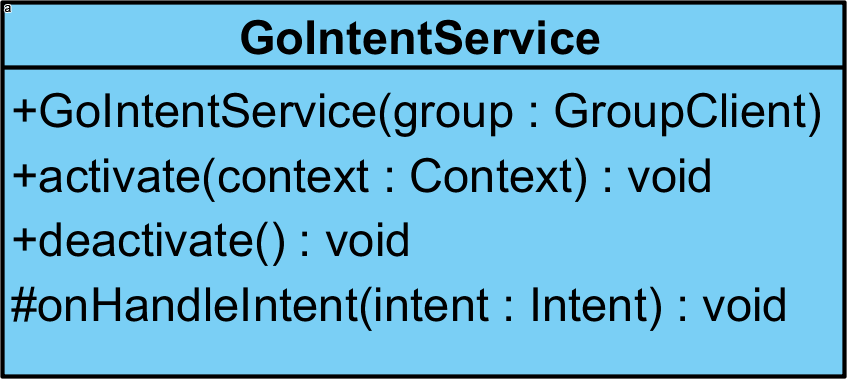
\includegraphics[scale = .3]{res/umlClasses/GoIntentService.png}
	\centering	
\end{figure}
Der GokIntentService kümmert sich um Netzwerkanfragen die den GoStatus, also Anfragen in regelmäßigen Zeitintervallen an den Server sendet und Koordinaten übermittelt. Dieser Service läuft im Hintergrund ab, um die Benutzeroberfläche nicht zu behindern.
\begin{enumerate}
	\item public GoIntentService(group: Group)
		Konstruktor für den IntentService.
	\item public activate(context: Context):void
		GoIntetnService wird aktiviert, wenn der GoStatus aktiviert wurde.
	\item public deactivate():void
		GoIntentService wird deaktiviert, wenn der GoStatus deaktiviert wurde.
	\item protected onHandleIntent(intent: Intent): void
		Für jede Netzwerkanfrage wird ein neuer Thread gestartet und es wird verhindert, dass Anfragen beim Drehen des Bildschirms verloren gehen.
\end{enumerate}

\paragraph{Database}
\begin{figure}[H]
	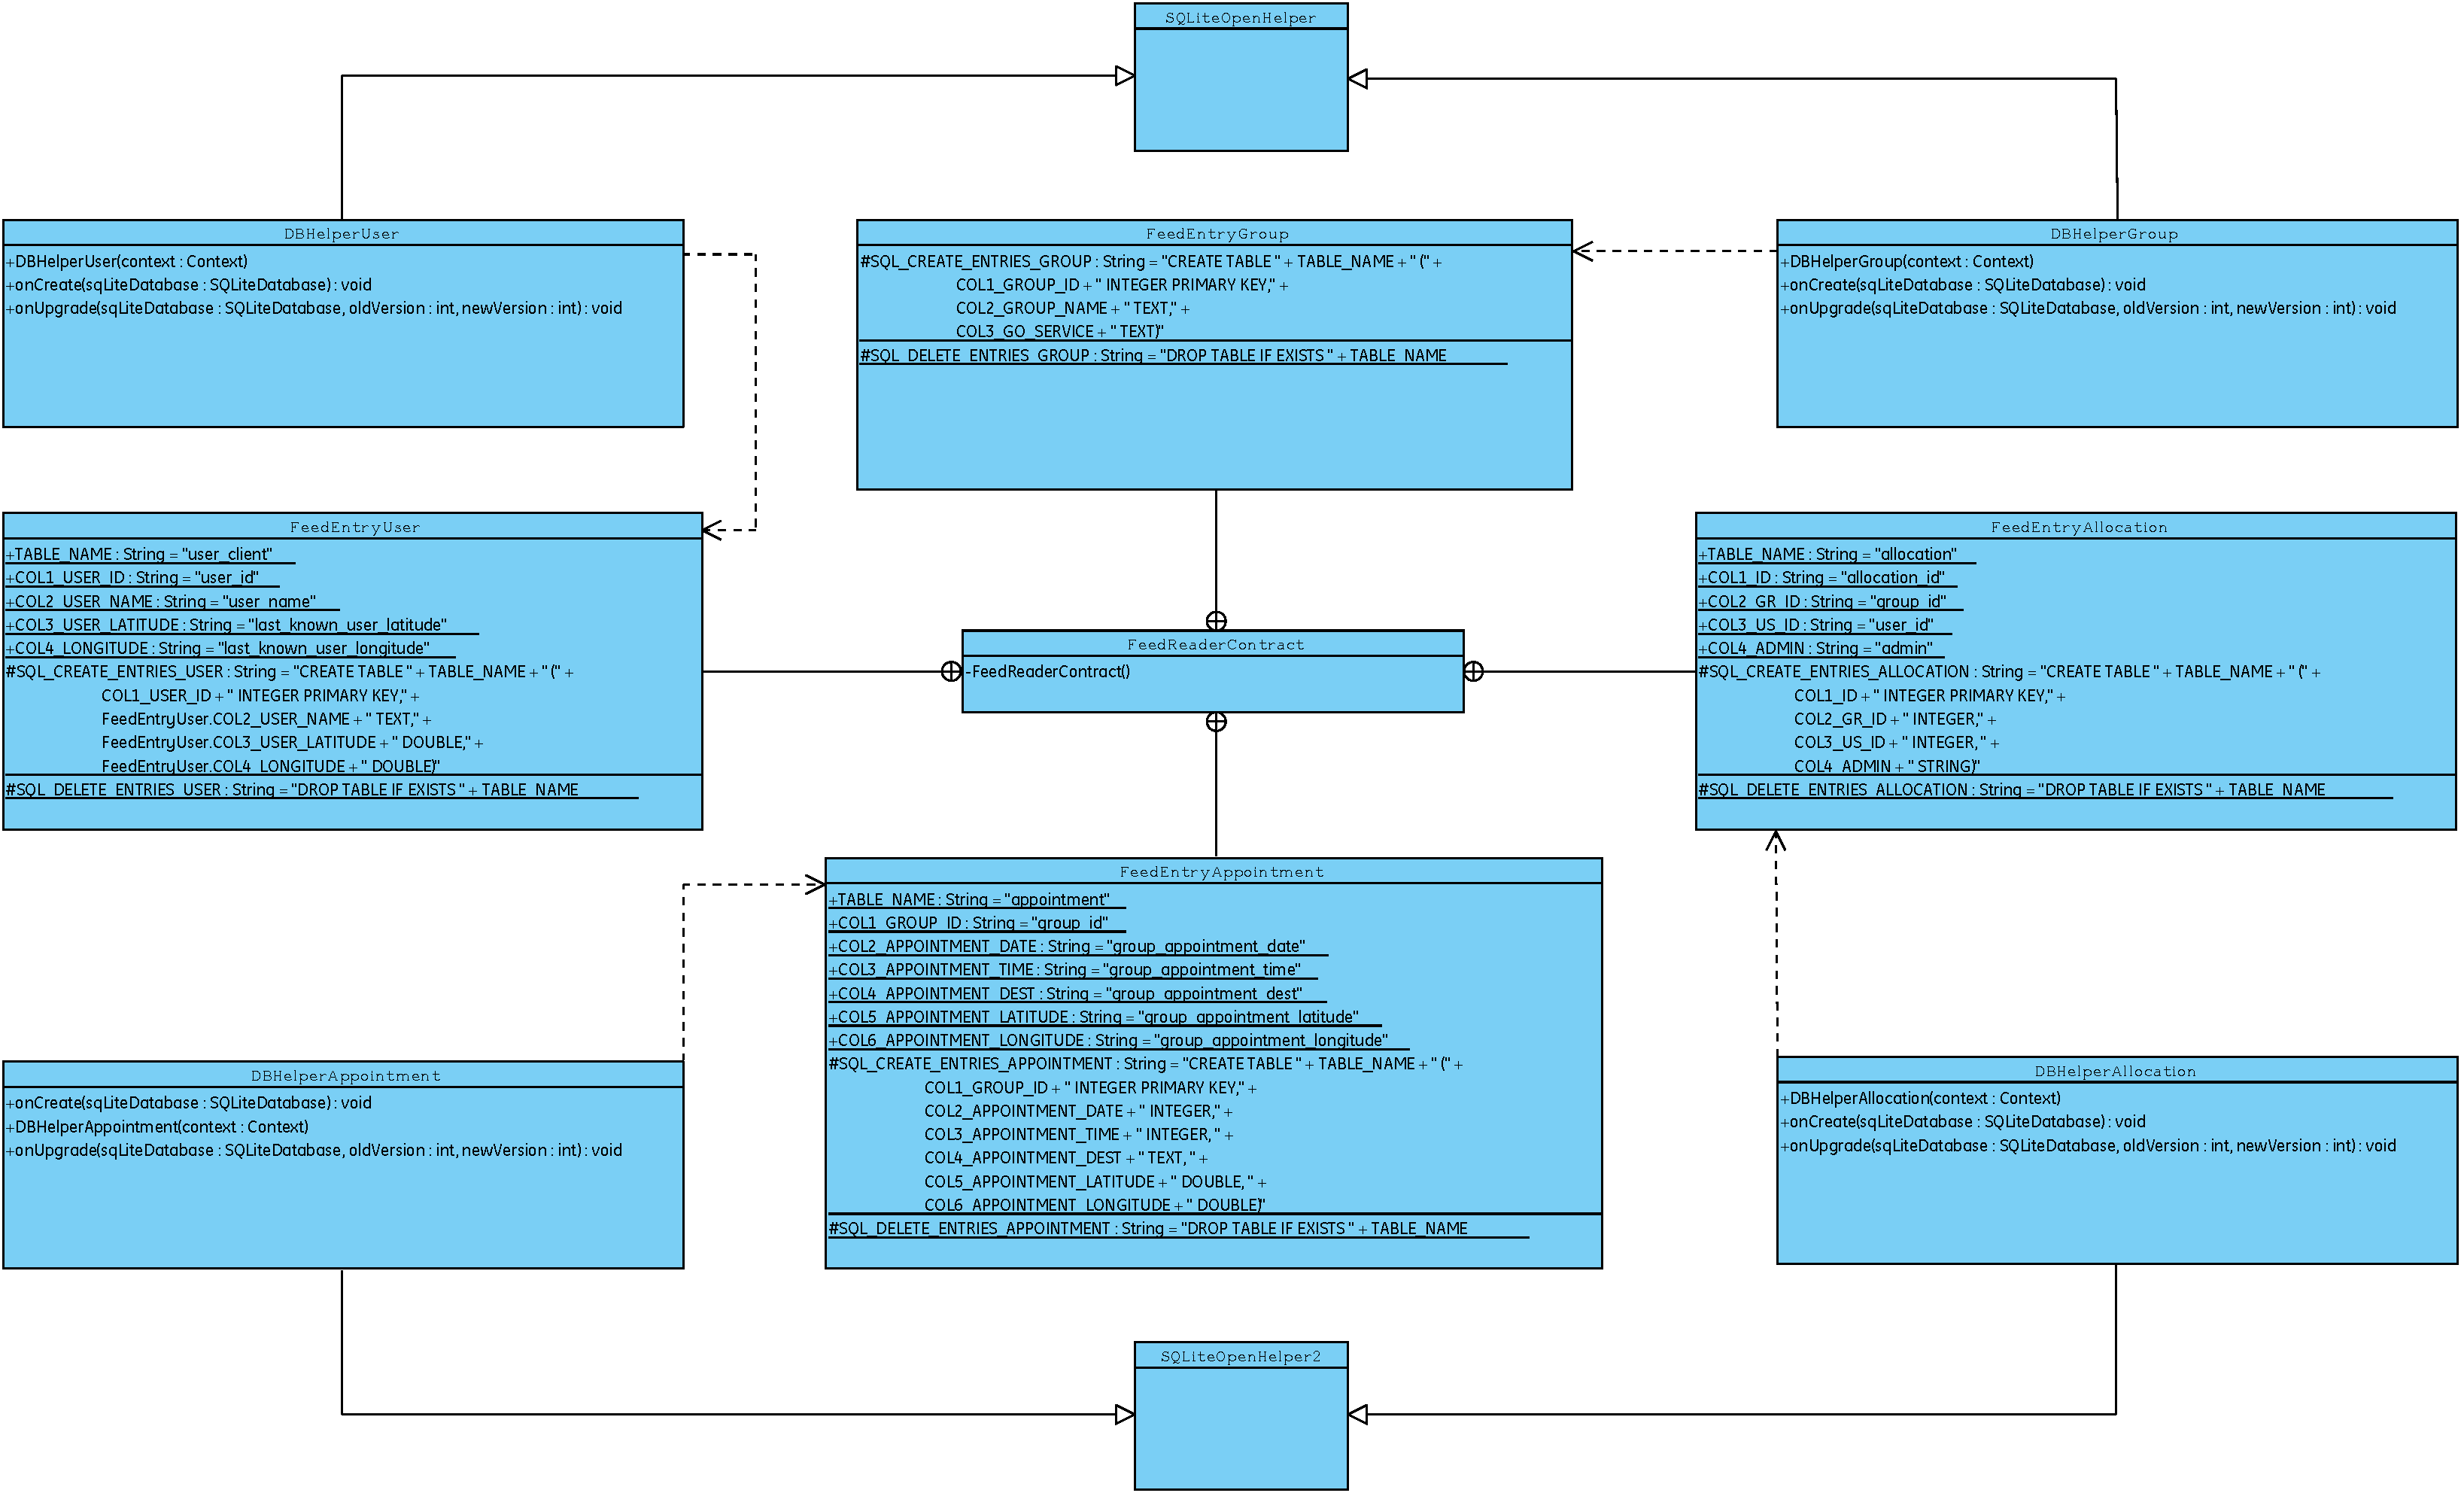
\includegraphics[scale = .3]{res/umlDiagramms/modelClientDatabase.pdf}
	\centering	
\end{figure}

\textbf{DBHelper}\\
Die vier nachfolgenden DBHelper erben ihren Konstruktor und ihre Methoden von SQLiteOpenHelper. 
\begin{enumerate}
	\item public DBHelperGroup(context: Context)\\
		Der Konstruktor definiert dabei den Namen und die Versionsnummer der Datenbank.
	\item public onCreate(sqLiteDatabase: SQLiteDatabase)\\
		Die SQLiteDatenbank wird mit den in FeedReaderEntry definierten Spalten aufgebaut, wenn sie das erste Mal aufgerufen wird.
	\item public onUpgrade(sqLiteDatabase: SQLiteDatabase, oldVersion: int, newVersion: int)\\
		Diese Methode wird verwendet, wenn man die Datenbank verändert hat. Dieser wird dann eine neue Versionsnummer zugeteilt.	
\end{enumerate}
\begin{figure}[H]
	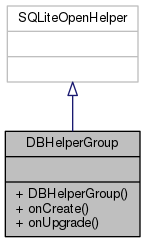
\includegraphics[scale = .5]{res/umlClasses/DBHelperGroup.png}
	\centering	
\end{figure}

\begin{figure}[H]
	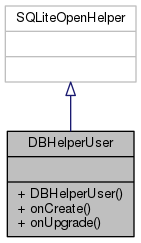
\includegraphics[scale = .5]{res/umlClasses/DBHelperUser.png}
	\centering
\end{figure}

\begin{figure}[H]
	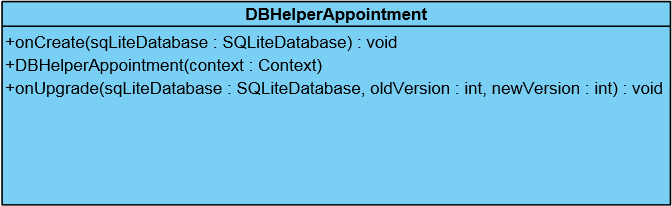
\includegraphics[scale = .58]{res/umlClasses/DBHelperAppointment.png}
	\centering
\end{figure}

\begin{figure}[H]
	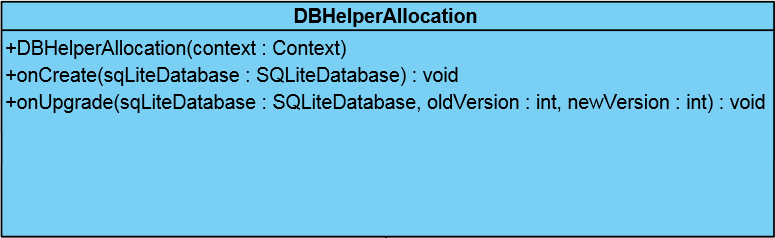
\includegraphics[scale = .5]{res/umlClasses/DBHelperAllocation.png}
	\centering
\end{figure}


\textbf{FeedReaderContract}
\begin{figure}[H]
	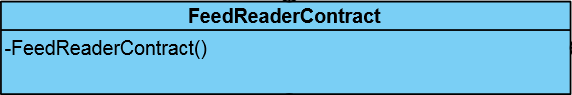
\includegraphics[scale = .5]{res/umlClasses/FeedReaderContract.png}
	\centering
\end{figure}
Die FeedReaderContract Klasse definiert in statischen Innenklassen wie die Tabellen der Datenbank aufgebaut sind. Jede der nachfolgenden FeedEntry Klassen implementiert dabei das Interface BaseColumns.

\begin{enumerate}
	\item public static final CREATE ENTRIES:String\\
		Legt die Spalten wenn die Tabelle generiert wird in genau dieser Reihenfolge an.
	\item public static final DELETE ENTRIES:Strning\\
		Löscht die zuvor definierten Spalteneinträge.
\end{enumerate}

\textbf{FeedEntyGroup}
\begin{figure}[H]
	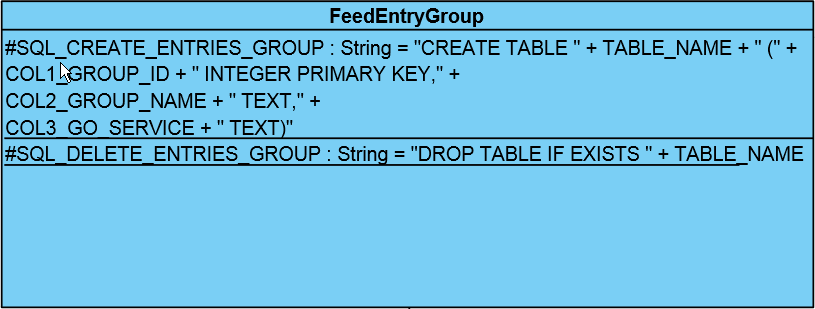
\includegraphics[scale = .5]{res/umlClasses/FeedEntryGroup.png}
	\centering
\end{figure}
Die Innenklasse FeedEntryGroup definiert den Namen und die Spalten der Tabelle, welche die Gruppen auf dem Client speichert. 
Dabei steht in der ersten Spalte die eindeutige Gruppen ID (welche die Zeilen eindeutig unterscheidbar macht), in der zweiten Spalte der eindeutige Gruppenname und in der dritten Spalte, ob der GoService des aktuellen Benutzers für diese Gruppe aktiviert oder deaktiviert ist.
Wenn eine Gruppe gelöscht wird, dann wird auch ihr Eintrag in der Datenbank gelöscht.

\textbf{FeedEntyUser}
\begin{figure}[H]
	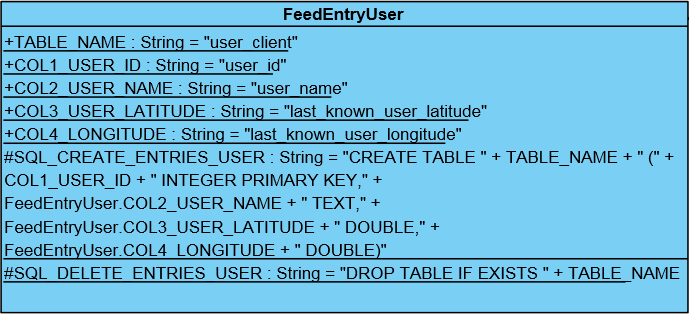
\includegraphics[scale = .6]{res/umlClasses/FeedEntryUser.png}
	\centering
\end{figure}
Die Innenklasse FeedEntryUser definiert den Namen und die Spalten der Tabelle, welche die Benutzer auf dem Client speichert. 
Dabei steht in der ersten Spalte die eindeutige Benutzer ID (welche die Zeilen eindeutig unterscheidbar macht), in der zweiten Spalte der Benutzername und in der dritten und vierten Spalte steht je ein Wert der zuletzt bekannten Gps Daten des jeweiligen Nutzers. 
Es werden nur Benutzer gespeichert mit denen der aktuelle Benutzer in mindestens einer gemeinsamen Gruppe ist.

\textbf{FeedEntyAppointment}
\begin{figure}[H]
	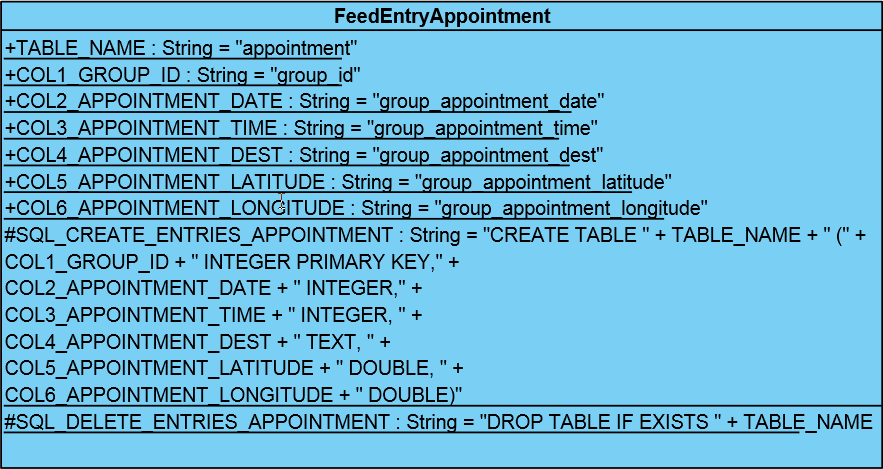
\includegraphics[scale = .5]{res/umlClasses/FeedEntryAppointment.png}
	\centering
\end{figure}
Die Innenklasse FeedEntryAppointment definiert den Namen und die Spalten der Tabelle, welche die Treffpunkte zu jeder Gruppe speichert. Jede Gruppe hat dabei nur eine Zeile, welche den Treffpunkt definiert. 
Dabei steht in der ersten Spalte die Gruppen id (welche die Zeilen eindeutig unterscheidbar macht), in der zweiten Spalte steht das Datum und in der dritten die Uhrzeit des Treffpunktes. In der vierten Spalte steht der Name des Zielortes und in der fünften und sechsten steht jeweils ein Wert der Gps Daten des Zielortes. 
Wenn sich der Treffpunkt der Gruppe ändert, dann werden die Werte des alten Treffpunktes überschrieben.
Sollte die die Gruppe des dazugehörigen Treffpunktes gelöscht werden, dann wird auch der Eintrag in dieser Tabelle gelöscht.

\textbf{FeedEntyAllocation}
\begin{figure}[H]
	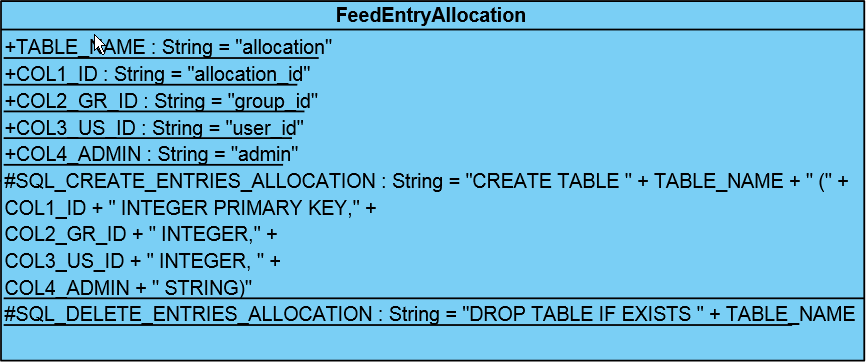
\includegraphics[scale = .5]{res/umlClasses/FeedEntryAllocation.png}
	\centering
\end{figure}
Die Innenklasse FeedEntryAllocation definiert den Namen und die Spalten der Tabelle, welche die jeweiligen Mitglieder jeder Gruppe speichert, in der der aktuelle Benutzer Mitglied ist. Zu jedem Mitglied wird vermerkt, ob dieses Administratorrechte hat.
Dabei steht in der ersten Spalte die Allocation id (welche die Zeilen eindeutig unterscheidbar macht und automatisch hochgezählt), in der zweiten Spalte steht die Gruppen id, in der dritten Spalte die Benutzer id und in der vierten Spalte, ob dieser Benutzer Gruppenadministrator ist oder nicht. 
Gruppen id wird für jedes Gruppenmitglied vermerkt, also kommt mehrmals vor, sobald mehr als ein Benutzer Mitglied dieser Gruppe ist.


\paragraph{ObjectStructure}

\begin{figure}[H]
	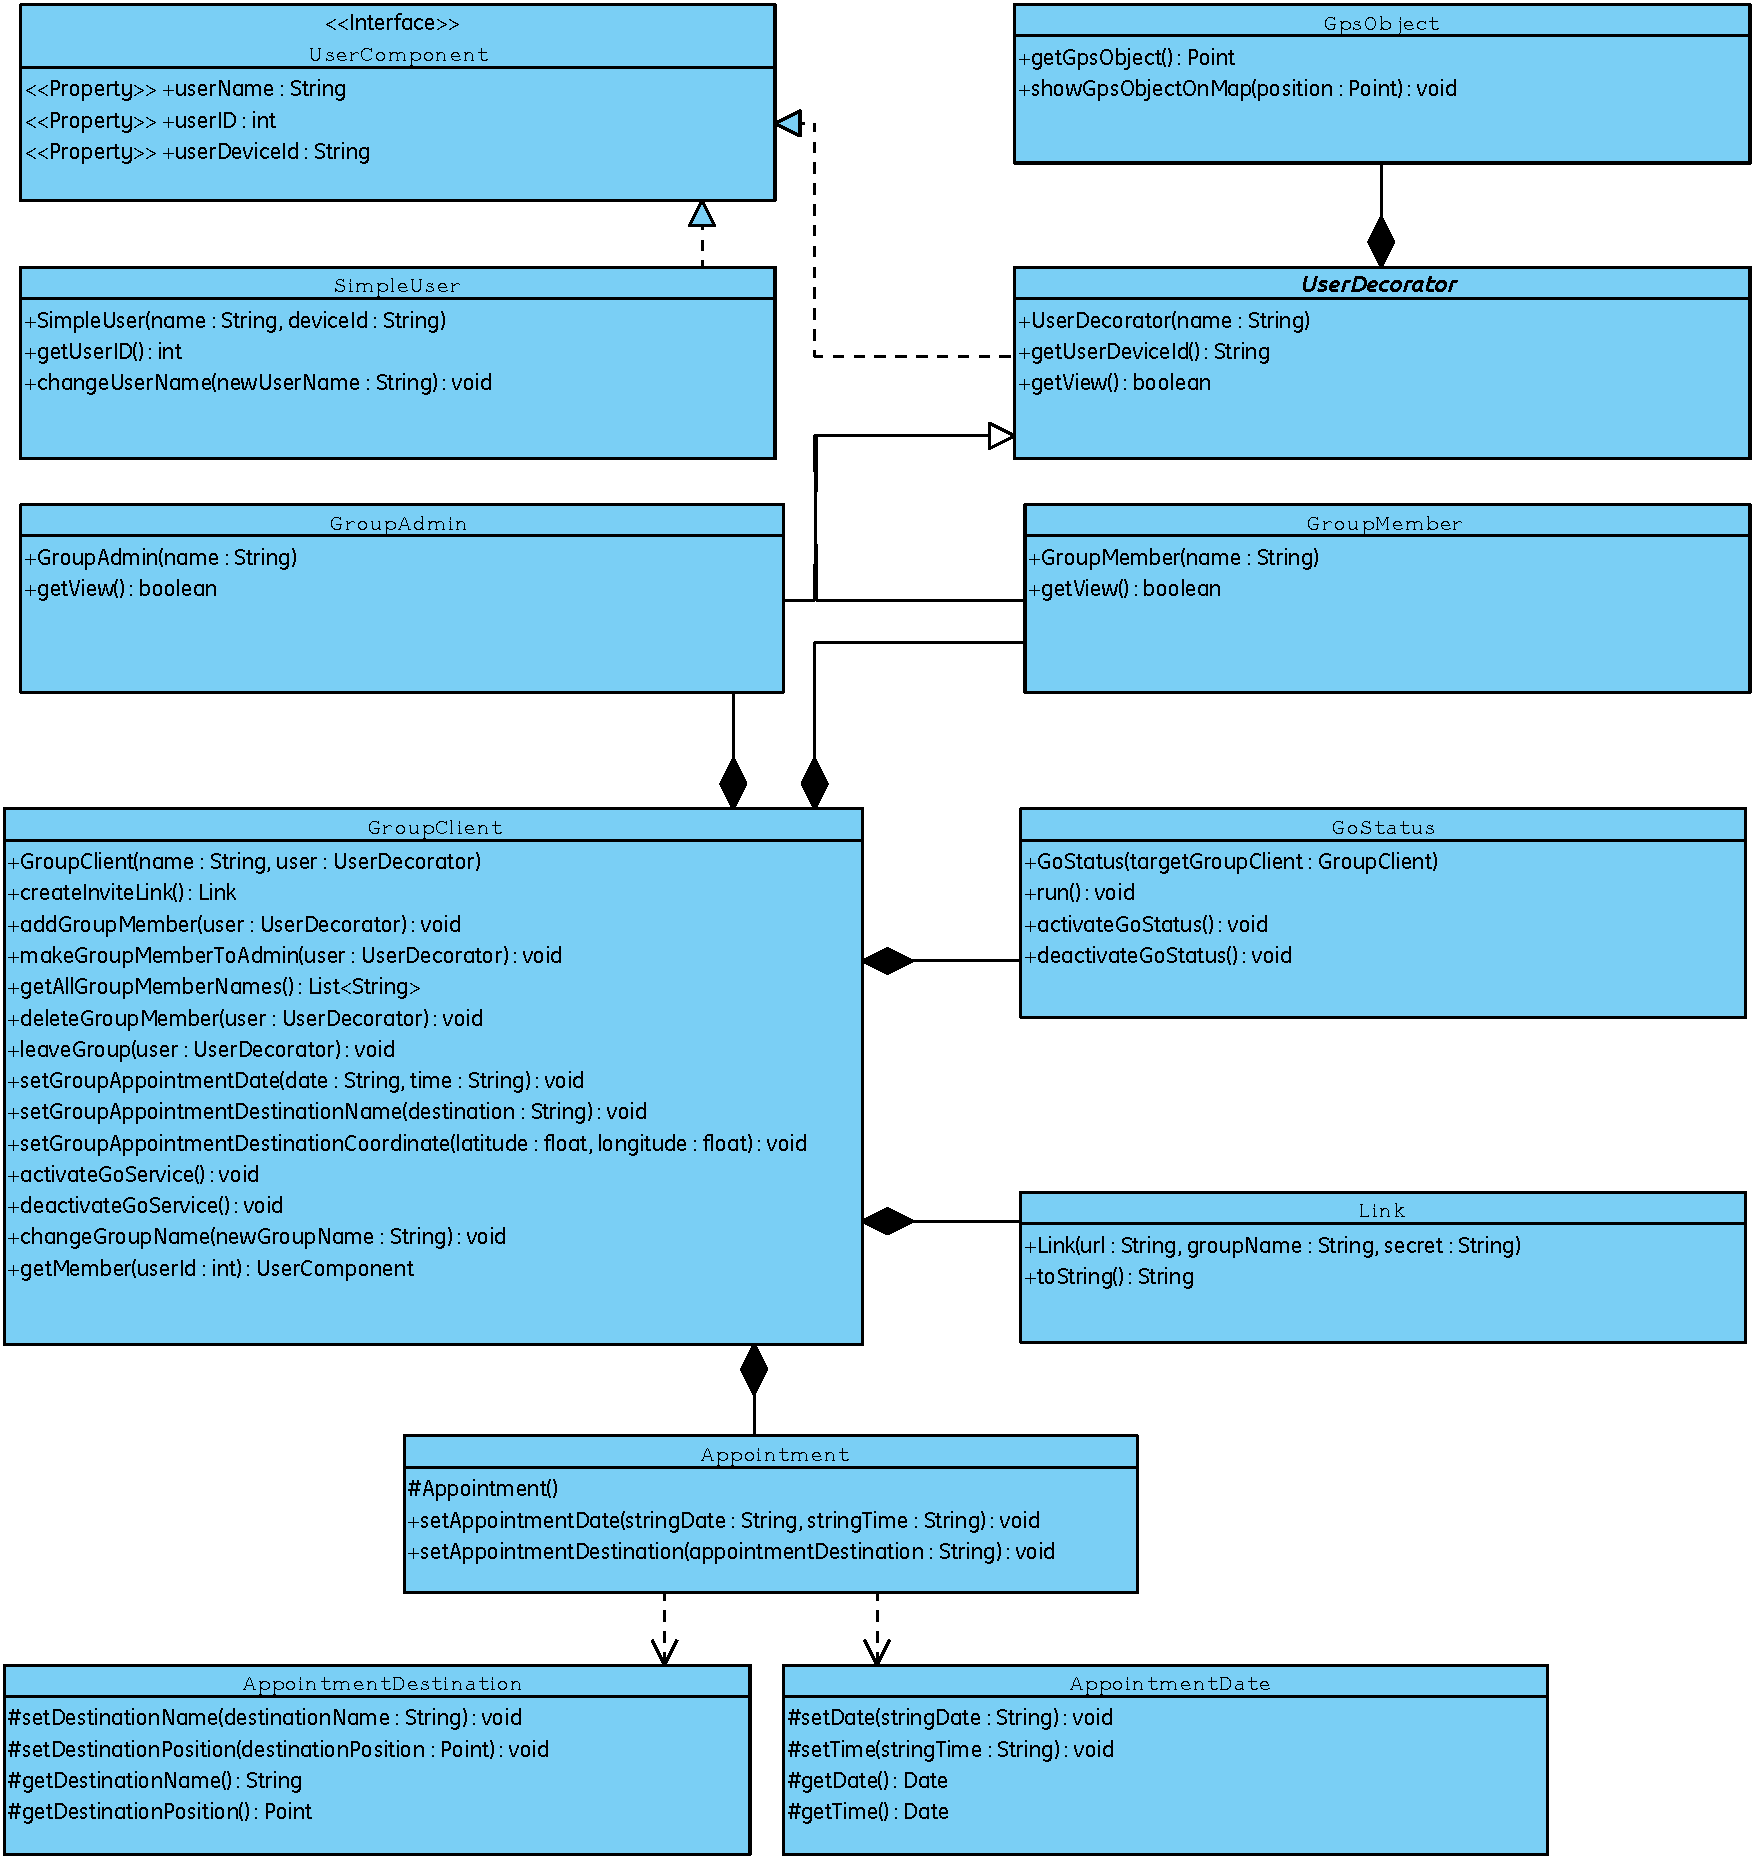
\includegraphics[scale = .5]{res/umlDiagramms/modelClientObjectStructure.pdf}
	\centering	
\end{figure}

\textbf{GroupClient}
\begin{figure}[H]
	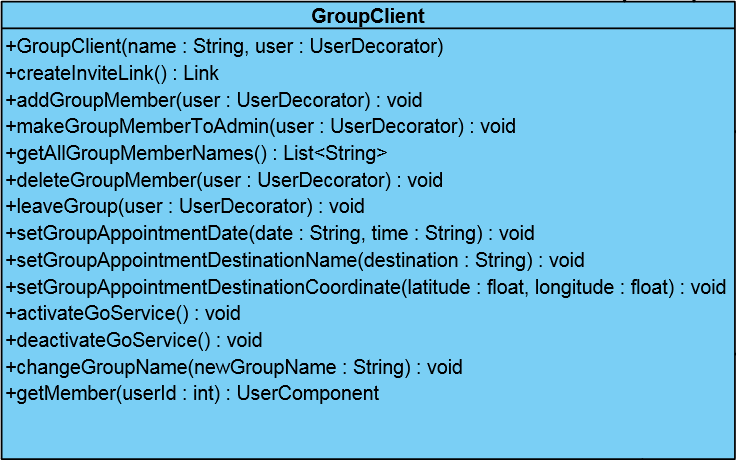
\includegraphics[scale = .5]{res/umlClasses/GroupClient.png}
	\centering
\end{figure}
Die Klasse GroupClient definiert wie eine Gruppe auf dem Client aufgebaut ist und welche Funktionalität ihr zur Verfügung steht.
\begin{enumerate}
	\item public GroupClient(name: String, user: UserDecorator)\\
		Konstruktor der einer neuen Gruppe einen eindeutigen Gruppennamen zuweist und den Ersteller als Gruppenadministrator festlegt.
	\item public createInviteLink():Link\\
		Um ein Gruppenmitglied hinzuzufügen, muss dieses über einen eindeutigen Link beitreten. Wird der Link ausgeführt wird man entweder zu GoApp weitergeleitet (hat App bereits installiert) oder wird dazu aufgefordert diese zu installieren. Der Link ist nicht mehr gültig sobald das Mitglied hinzugefügt wurde. Man muss Administrator sein um diese Funktion verwenden zu können.
	\item public addGroupMember(user: UserDecorator)\\
		Ein Mitglied wird der Gruppe hinzugefügt.
	\item public makeGroupMemberToAdmin(user: UserDecorator)\\
		Ein Gruppenmitglied wird vom Administrator zum Gruppenadministrator gemacht.
	\item public getAllGroupMemberNames():List<String>\\
		Alle Namen der Mitglieder einer Gruppe werden zurückgegeben.
	\item public deleteGroupMember(user:UserDecorator)\\
		Ein Gruppenmitglied wird aus der Gruppe durch den Administrator entfernt.
	\item public leaveGroup(user:UserDecorator)\\
		Ein Mitglied verlässt die Gruppe.
	\item public activateGoService()\\
		Der aktuelle Benutzer aktiviert seinen GoStatus und übermittelt seine GPS Daten an die Gruppe (GPS muss eingeschalten sein).
	\item public deactivateGoService()\\
		Der aktuelle Benutzer deaktiviert seinen GoStatus und wird nicht mehr verfolgt.
	\item public changeGroupName(newGroupName:String)\\
		Der Gruppenadministrator benennt die Gruppe zu einem anderen eindeutigen Namen um.
	\item public getGroupID():int \\
		Die Gruppen Id wird zurückgegeben
	\item public getGroupName():String\\
		Der Gruppenname wird zurückgegeben 
	\item public getGoStatus():GoStatus \\
		Der GoStatus wird zurückgegeben
	\item public getAppointment():Appointment \\
		Das Appointment wird zurückgegeben
	\item public getMember(userId: int):UserComponent \\
		Der Typ des aktuellen Benutzers einer Gruppe (Gruppenmitglied oder Administrator)wird zurückgegeben, um die Ansicht der Gruppe auf seine ihm zugänglichen Funktionen zu beschränken/ erweitern.
\end{enumerate}

\textbf{UserComponent}
\begin{figure}[H]
	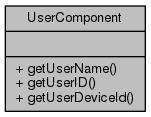
\includegraphics[scale = .5]{res/umlClasses/UserComponent.png}
	\centering
\end{figure}
Dieses Interface ist die erste Komponente des Decorator pattern und definiert grundlegende Funktionen des Benutzers die jederzeit aufgerufen werden können. 

Mit getUserId() kann der Benutzer von anderen Gruppenmitgliedern unterschieden werden, da der Benutzername nicht eindeutig sein muss, die Id aber schon.
Mit getUserDeviceId() kann der Benutzer auf dem Server angelegt werden. Jede Gerätenummer kann nur einmal auf dem Server vorkommen, um Missbrauch der GoApp vorzubeugen.
\begin{enumerate}
	\item public getUserName():String\\
		Benutzername des aktuellen Benutzers kann in der GoApp visualisiert werden.
	\item public getUserID():int\\
		Mit der Benutzer Id kann sich der aktuelle Benutzer unter den anderen Gruppenmitglieder identifizieren.
	\item public getUserDeviceID():String\\
		Die Device Id wird auf dem Server zusammen mit den anderen zwei Werten gespeichert, um einem Endgerät nur einen Benutzer zu erlauben, um Missbrauch zu vermeiden.
\end{enumerate}

\textbf{SimpleUser}
\begin{figure}[H]
	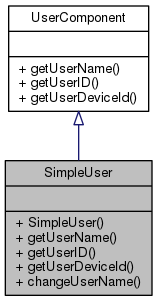
\includegraphics[scale = .5]{res/umlClasses/SimpleUser.png}
	\centering
\end{figure}
Die SimpleUser Klasse implementiert das UserComponent Interface. Der Benutzer ist ein SimpleUser Objekt, wenn er nicht in der Gruppenansicht ist und so weder einem Gruppenadministrator noch einem Gruppenmitglied entspricht.
\begin{enumerate}
	\item public getUserName():String\\
		Siehe UserComponent.
	\item public getUserID():int\\
		Siehe UserComponent.
	\item public getUserDeviceID():String\\
		Siehe UserComponent.
	\item public changeUserName(newUserName: String)\\
	Der aktuelle Benutzer kann seinen Benutzernamen nachträglich ändern.
\end{enumerate}

\textbf{UserDecorator}
\begin{figure}[H]
	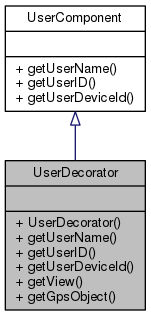
\includegraphics[scale = .5]{res/umlClasses/UserDecorator.png}
	\centering
\end{figure}
Die UserDecorator Klasse ist eine abstrakte Klasse, die wie SimpleUser das UserComponent Interface implementiert. 
\begin{enumerate}
	\item public getUserName():String\\
		Siehe UserComponent.
	\item public getUserID():int\\
		Siehe UserComponent.
	\item public getUserDeviceID():String\\
		Siehe UserComponent.
	\item public getView():boolean\\
		Mit dieser Methode wird bestimmt welche Gruppenansicht der aktuelle Benutzer sieht (die für ein Gruppenmitglied oder die für einen Gruppenadministrator mit zusätzlichen Funktionen).
	\item public getGpsObject():GpsObject\\
		Die Gps Daten des aktuellen Benutzers werden zurück gegeben.
\end{enumerate}

\textbf{GroupAdmin}
\begin{figure}[H]
	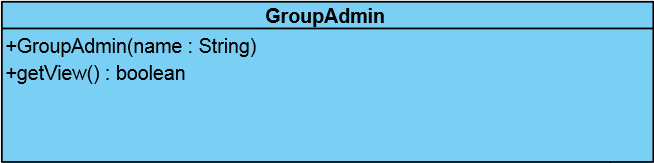
\includegraphics[scale = .5]{res/umlClasses/GroupAdmin.png}
	\centering
\end{figure}
Der Gruppenadministrator unterscheidet sich vom Gruppenmitglied in sofern, dass ihm weitaus mehr Funktionen zur Verfügung stehen, wie Mitglieder hinzufügen/ entfernen und Treffpunkte festlegen.
\begin{enumerate}
	\item public GroupAdmin(name: String)\\
		Konstruktor für einen Gruppenadministrator.
	\item public getView():boolean\\
		Siehe UserDecorator.
\end{enumerate}

\textbf{GroupMember}
\begin{figure}[H]
	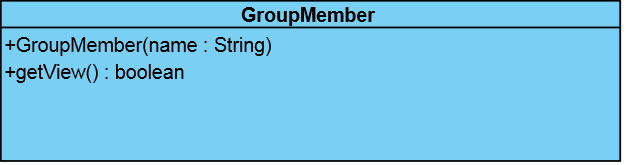
\includegraphics[scale = .5]{res/umlClasses/GroupMember.png}
	\centering
\end{figure}
Das Gruppenmitglied unterscheidet sich vom Gruppenadministrator in sofern, dass ihm die Gruppe betreffend kaum Funktionen zur Verfügung stehen.  
\begin{enumerate}
	\item public GroupMember(name: String)\\
		Konstruktor für einen Gruppenmitglied.
	\item public getView():boolean\\
		Siehe UserDecorator.
\end{enumerate}

\textbf{GoStatus}
\begin{figure}[H]
	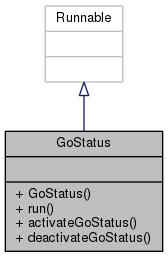
\includegraphics[scale = .5]{res/umlClasses/GoStatus.png}
	\centering
\end{figure}
Der GoStatus bestimmt darüber in welchen Abständen die Position des aktuellen Benutzers an die anderen Gruppenmitglieder übermittelt wird.
\begin{enumerate}
	\item public GoStatus(targetGroupClient: GroupClient)\\
		Konstruktor für den GoStatus wird für jede Gruppe für den aktuellen Benutzer definiert.
	\item public run()\\
		Periodisch bei aktivierten GoStatus der Standort an die Gruppenmitglieder weitergeleitet.
	\item public activateGoStatus()\\
		GoStatus und Gps Tracking aktivieren.
	\item public deactivateGoStatus()\\
		Gps Tracking deaktivieren.
\end{enumerate}

\textbf{Link}
\begin{figure}[H]
	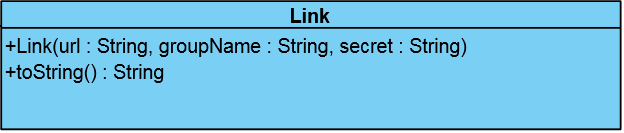
\includegraphics[scale = .5]{res/umlClasses/Link.png}
	\centering
\end{figure}
Mit dem Link kann man andere Mitglieder 
\begin{enumerate}
	\item public Link(url: String, groupName: String , secret: String)\\
		Konstruktor für einen Link. Ein Gruppenlink besteht aus den gelisteten drei Komponenten. Durch den Gruppennamen lässt sich das Mitglied welches den Link betätigt zu derjenigen Gruppe hinzufügen und das sercret verhindert, dass der Link leicht regenerierbar ist.
	\item public toString():String\\
		Der Link wird wieder in seine einzelne Komponenten sortiert.
\end{enumerate}

\textbf{GpsObject}
\begin{figure}[H]
	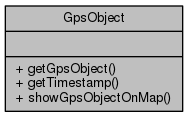
\includegraphics[scale = .5]{res/umlClasses/GpsObject.png}
	\centering
\end{figure}
Das GpsObject gibt an in welcher Form die Gps Daten übermittelt werden.
\begin{enumerate}
	\item public getGpsObject():Point\\
		Der Konstruktor für das GpsObject definiert ein neuen Point der aus einem Längen und einem Breitengrad besteht. 
	\item public getTimestamp():String \\
		Timestamp gibt zurück, wie alt der zuletzt ermittelte Standort ist.
\end{enumerate}

\textbf{Appointment}
\begin{figure}[H]
	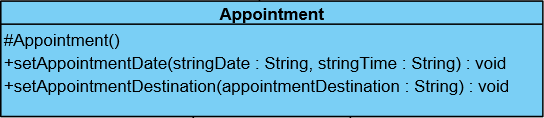
\includegraphics[scale = .6]{res/umlClasses/Appointment.png}
	\centering
\end{figure}
Appointment fasst alle Informationen zusammen die es über den Treffpunkt zu speichern gibt.
\begin{enumerate}
	\item protected Appointment()\\	
		Konstruktor für ein Appointment welches beim Erstellen einer Gruppe default Werte für Datum, Uhrzeit und Ort definiert.
	\item public setAppointmentDate(String stringDate, String stringTime)\\
		Datum und Uhrzeit des Treffens ändern.
	\item getAppointmentDate():AppointmentDate \\
		Datum und Uhrzeit des Appointments zurückgeben.
	\item public setAppointmentDestination(String appointmentDestination)\\
		Über den Namen/Adresse oder über die Position auf der Karte einen Zielort setzen.
	\item public getAppointmentDestination():AppointmentDestination\\
		Den Zielortes des Treffpunktes zurückgeben.
\end{enumerate}

\textbf{AppointmentDate}
\begin{figure}[H]
	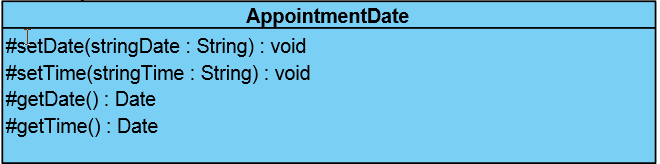
\includegraphics[scale = .5]{res/umlClasses/AppointmentDate.png}
	\centering
\end{figure}
AppointmentDate legt fest wie Datum und Uhrzeit formatiert werden.
\begin{enumerate}
	\item protected setDate(stringDate: String)\\
		Ein Datum festlegen.
	\item protected setTime(stringTime: String)\\
		Eine Uhrzeit festlegen.
	\item protected getDate():Date \\
		Das Datum zurückgeben.
	\item protected getTime():Date \\
		Die Uhrzeit zurückgeben.
\end{enumerate}

\textbf{AppointmentDestination}
\begin{figure}[H]
	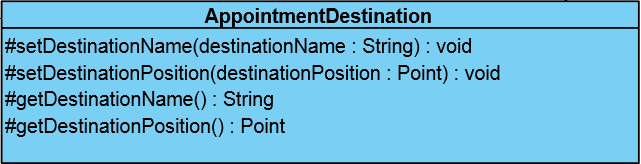
\includegraphics[scale = .5]{res/umlClasses/AppointmentDestination.png}
	\centering
\end{figure}
AppointmentDestination legt fest wie Name und Position des Zielortes definiert sind.
\begin{enumerate}
	\item protected setDestinationName(destinationName:String)\\
		Den Zielort über den Namen/ die Adresse bestimmen.
	\item protected setDestinationPosition(destinationPosition:Point)\\
		Den Zielort über eine Position auf der Karte bestimmen.
	\item protected getDestinationName():String \\
		Den Zielortnamen zurückgeben.
	\item protected getDestinationPosition():Point \\
		Die Zielortposition zurückgeben.
\end{enumerate}


\subsubsection{ClientController}

\textbf{NetworkIntentService}

\paragraph{Database}

\textbf{Services}
Die folgenden Service Klassen stellen die grundlegenden Funktionen zur Verfügung, mit welchen auf die Daten der in den Innenklassen von FeedReaderContract definierten Tabellen der Datenbank zugegriffen werden kann. Dabei können Daten hinzugefügt (insert), gelesen (read), gelöscht (delete) und verändert (update) werden.
Weitere Details dazu, wie die jeweilige Datenbanken aufgebaut sind, finden sie in FeedEntryGroup, FeedEntryUser, FeedEntryAppointment, FeedEntryAllocation.

\begin{figure}[H]
	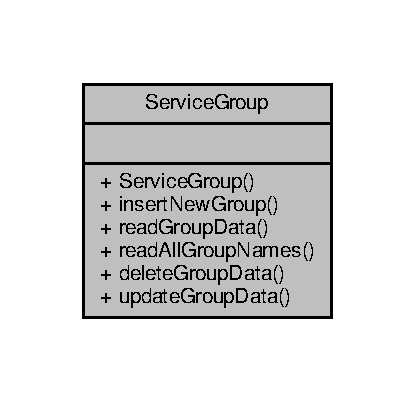
\includegraphics[scale = 1]{res/umlClasses/service_group__coll__graph.pdf}
	\centering
\end{figure}
In der Datenbank auf die ServiceGroup zugreift, werden die Gruppen gespeichert und ob der aktuelle Nutzer der Go-App für diese spezielle Gruppe seinen Go-Button aktiviert hat oder nicht. 
\begin{enumerate}
	\item public ServiceGroup(context: Context)\\
		Konstruktor, dem den Kontext der Applikation mitgegeben wird.
	\item public insertNewGroup(groupClient: GroupClient):boolean\\
		Eine neue Gruppe wird der Datenbank hinzugefügt und der GoStatus des Erstellers auf false gesetzt.
	\item public readGroupData(groupID: int):GroupClient \\
		Informationen über Gruppenname und GoStatus lesen. 
	\item public readAllGroupNames():List<String>\\
		Alle Gruppen in denen der aktuelle Benutzer Mitglied ist werden zurückgegeben.
	\item public deleteGroupData(groupID: int):boolean\\
		Eine Gruppe wird aus der Datenbank gelöscht.
	\item public updateGroupData(groupClient: GroupClient ):boolean\\
		Gruppendaten werden aktualisiert, wenn sich der Gruppenname oder der GoStatus ändert.
\end{enumerate}

\begin{figure}[H]
	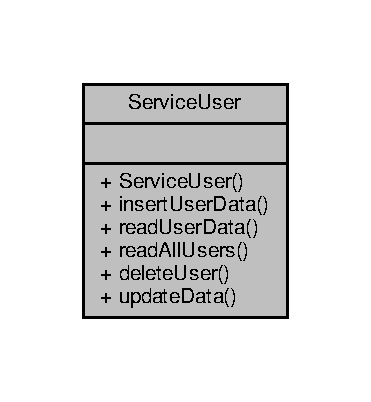
\includegraphics[scale = 1]{res/umlClasses/service_user__coll__graph.pdf}
	\centering
\end{figure}
In der Datenbank auf die ServiceUser zugreift ist der Name und die zuletzt bekannte Position des Benutzers gespeichert, welche bei neuen Informationen angepasst werden. 
\begin{enumerate}
	\item public ServiceUser(context: Context)\\
		Konstruktor, dem den Kontext der Applikation mitgegeben wird.
	\item public insertUserData(UserDecorator user):boolean\\
		Ein neuer Benutzer wird der Datenbank hinzugefügt, sobald dieser mit dem aktuellen Benutzer in einer Gruppe ist.
	\item public readUserData(userID: int):UserDecorator\\
		Inforamtionen über Benutzername und Position eines Benutzers können gelesen werden.
	\item public readAllUsers():List<UserDecorator> \\
		Alle Benutzernamen mit denen der aktuelle Benutzer in einer Gruppe ist lesen.
	\item public deleteUser(userID: int):boolean\\
		Einen Benutzer von der Datenbank entfernen.
	\item public updateData(userID: int):boolean\\
		Benutzerdaten anpassen, wenn sich Name oder Position geändert haben.
\end{enumerate}

\begin{figure}[H]
	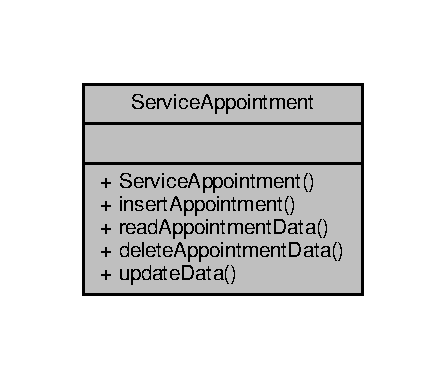
\includegraphics[scale = 1]{res/umlClasses/service_appointment__coll__graph.pdf}
	\centering
\end{figure}
In der Datenbank auf die ServiceAppointment zugreift, wird zu jeder Gruppe das aktuelle Treffen gespeichert und verändert, sobald ein neues existiert.
\begin{enumerate}
	\item public ServiceAppointment(context: Context)\\
		Konstruktor, dem den Kontext der Applikation mitgegeben wird.
	\item public insertAppointment(groupID: int, appointment: Appointment):boolean\\
		Wird aufgerufen wenn eine neue Gruppe erstellt wird. Dabei wird ein default Appointment initialisiert.
	\item public readAppointmentData(groupID: int):Appointment \\
		Informationen über Datum, Uhrzeit, Zielortname und Zielortposition können abgerufen werden.
	\item public deleteAppointmentData(groupID: int):boolean \\
		Wenn eine Gruppe gelöscht wird, wir auch das dazugehörige Appointment gelöscht.
	\item public updateData(groupID: int, appointment: Appointment):boolean \\
		Das Appointment wird angepasst, sobald es geändert wird.
\end{enumerate}

\begin{figure}[H]
	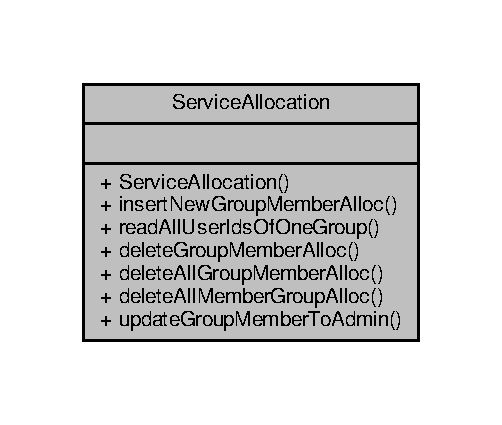
\includegraphics[scale = 1]{res/umlClasses/service_allocation__coll__graph.pdf} 
	\centering
\end{figure}
In der Datenbank auf die ServiceAllocation zugreift, wird die Verbindung zwischen Gruppen und Gruppenmitgliedern bzw. Administratoren gespeichert. 
\begin{enumerate}
	\item public (context: Context):ServiceAllocation\\
		Konstruktor, dem den Kontext der Applikation mitgegeben wird.
	\item public insertNewGroupMemberAlloc(groupID: int , userID: int):boolean\\
		Wenn ein neues Mitglied einer Gruppe hinzugefügt wird, dann wird diese Verbindung hier eingetragen.
	\item public readAllUserIdsOfOneGroup(groupID: int ):List<Integer> \\
		Um alle Mitglieder einer Gruppe zu bekommen, müssen dafür alle Benutzer Id's mit derselben Gruppen Id zurückgegeben werden.
	\item public deleteGroupMemberAlloc(groupid: int, userId: int):boolean \\
		Wird ein Gruppenmitglied aus einer Gruppe entfernt, so wird auch die Verbindung von diesem zur Gruppe gelöscht.
	\item public deleteAllGroupMemberAlloc(groupId: int):boolean \\
		Wird eine Gruppe gelöscht, so werden alle Verbindungen zu Benutzern dieser Gruppe gelöscht.
	\item public updateGroupMemberToAdmin(groupId: int , userID: int):boolean \\
		Wird ein Gruppenmitglied zum Administrator gemacht, dann wird dies in der Datenbank angepasst.
\end{enumerate}
	

\paragraph{ObjectStructure}

In Account- und GroupHandler werden allgemeine Funktionen definiert, die nicht selbst vom GroupClient oder von Unterklassen von UserComponent ausgeführt werden können, sondern eine übergeordnete Position benötigen.

\textbf{AccountHandler}
\begin{figure}[H]
	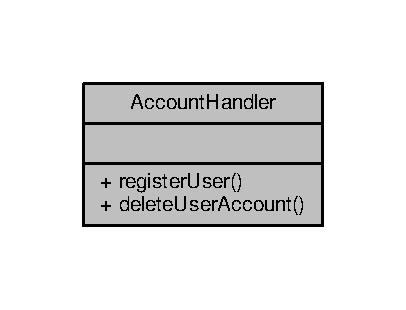
\includegraphics[scale = 1]{res/umlClasses/account_handler__coll__graph.pdf}
	\centering
\end{figure}
Die AccountHandler Klasse handelt das Registrieren und löschen vom aktuellen Benutzer ab.
\begin{enumerate}
	\item public registerUser(userName: String, deviceID: String)\\
		Ein neuer Benutzer registriert sich mit einem Namen und seiner Gerätenummer. Dieser wird zunächst als SimpleUser Objekt angelegt und mit der Gerätenummer auf dem Server gespeichert, um Missbrauch zu verhindern.
	\item public deleteUserAccount(user: UserDecorator)\\
		Löscht ein Benutzer seinen Account, wird er von der Datenbank gelöscht.
\end{enumerate}

\textbf{GroupHandler}
\begin{figure}[H]
	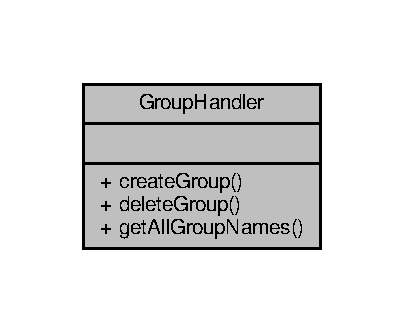
\includegraphics[scale = 1]{res/umlClasses/group_handler__coll__graph.pdf}
	\centering
\end{figure}
Die GroupHandler Klasse handelt das Erstellen und Löschen von Gruppen ab.
\begin{enumerate}
	\item public createGroup(groupName: String, user: UserDecorator)\\
		Eine neue Gruppe wird erstellt, mit einem eindeutigen Gruppennamen und mit dem Ersteller als Administrator.
	\item public deleteGroup(GroupClient groupClient)\\
		Eine Gruppe wird gelöscht und alle ihre Mitglieder entfernt.
\end{enumerate}



\subsection{Serverseitig}
\makeatletter
\renewcommand\paragraph{\@startsection{paragraph}{4}{\z@}%
{-2.5ex\@plus -1ex \@minus -.25ex}%
{1.25ex \@plus .25ex}%
{\normalfont\normalsize\bfseries}}
\makeatother
\setcounter{secnumdepth}{5} % how many sectioning levels to assign numbers to
\setcounter{tocdepth}{5}

\subsubsection{Servlets}
Die Tomcat-Servlets bilden zusammen einen Webservice in Anlehnung an einen \\
REST-Webservice (Representational State Transfer). \\
Im MVC-Paradigma würden sie in die Kategorie Controller fallen.\\
Die Servlets sind in verschiedene Aufgabenbereiche unterteilt. Alle Servlets \\erben von BaseServlet, was wiederum von HttpServlet erbt.
Die genaue Art der Anfrage wird über den QueryString der HttpServletRequest bestimmt.\\
Alle Anfragen werden in Form von JSON über die HTTP-POST methode übergeben.\\
In der doPost() Methode der Servlets werden sie bearbeitet.
die doGet() Methode wird bei einer HTTP-GET request aufgerufen. \\
Sie liefert Informationen
über den Zustand des Servlets, bzw. leitet den Nutzer weiter, falls er die Anfrage von einem Webbrowser aus sendet.\\
Über einen POST erhaltene Daten werden als JSON String interpretiert und via \\Jackson API auf Request-Objekte abgebildet.\\
Innerhalb des Request-Objekts sind Benutzer und Gruppen nur durch ID und Name spezifiziert.
Die zugehörigen Objekte werden aus der Datenbank angefordert. \\Name und ID dienen dabei als Schlüssel.\\
\\
Das GroupServlet als Beispiel zur server-internen Bearbeitung von Anfragen:
\\

\begin{figure}[h]
     \centering
     \hspace*{-2cm}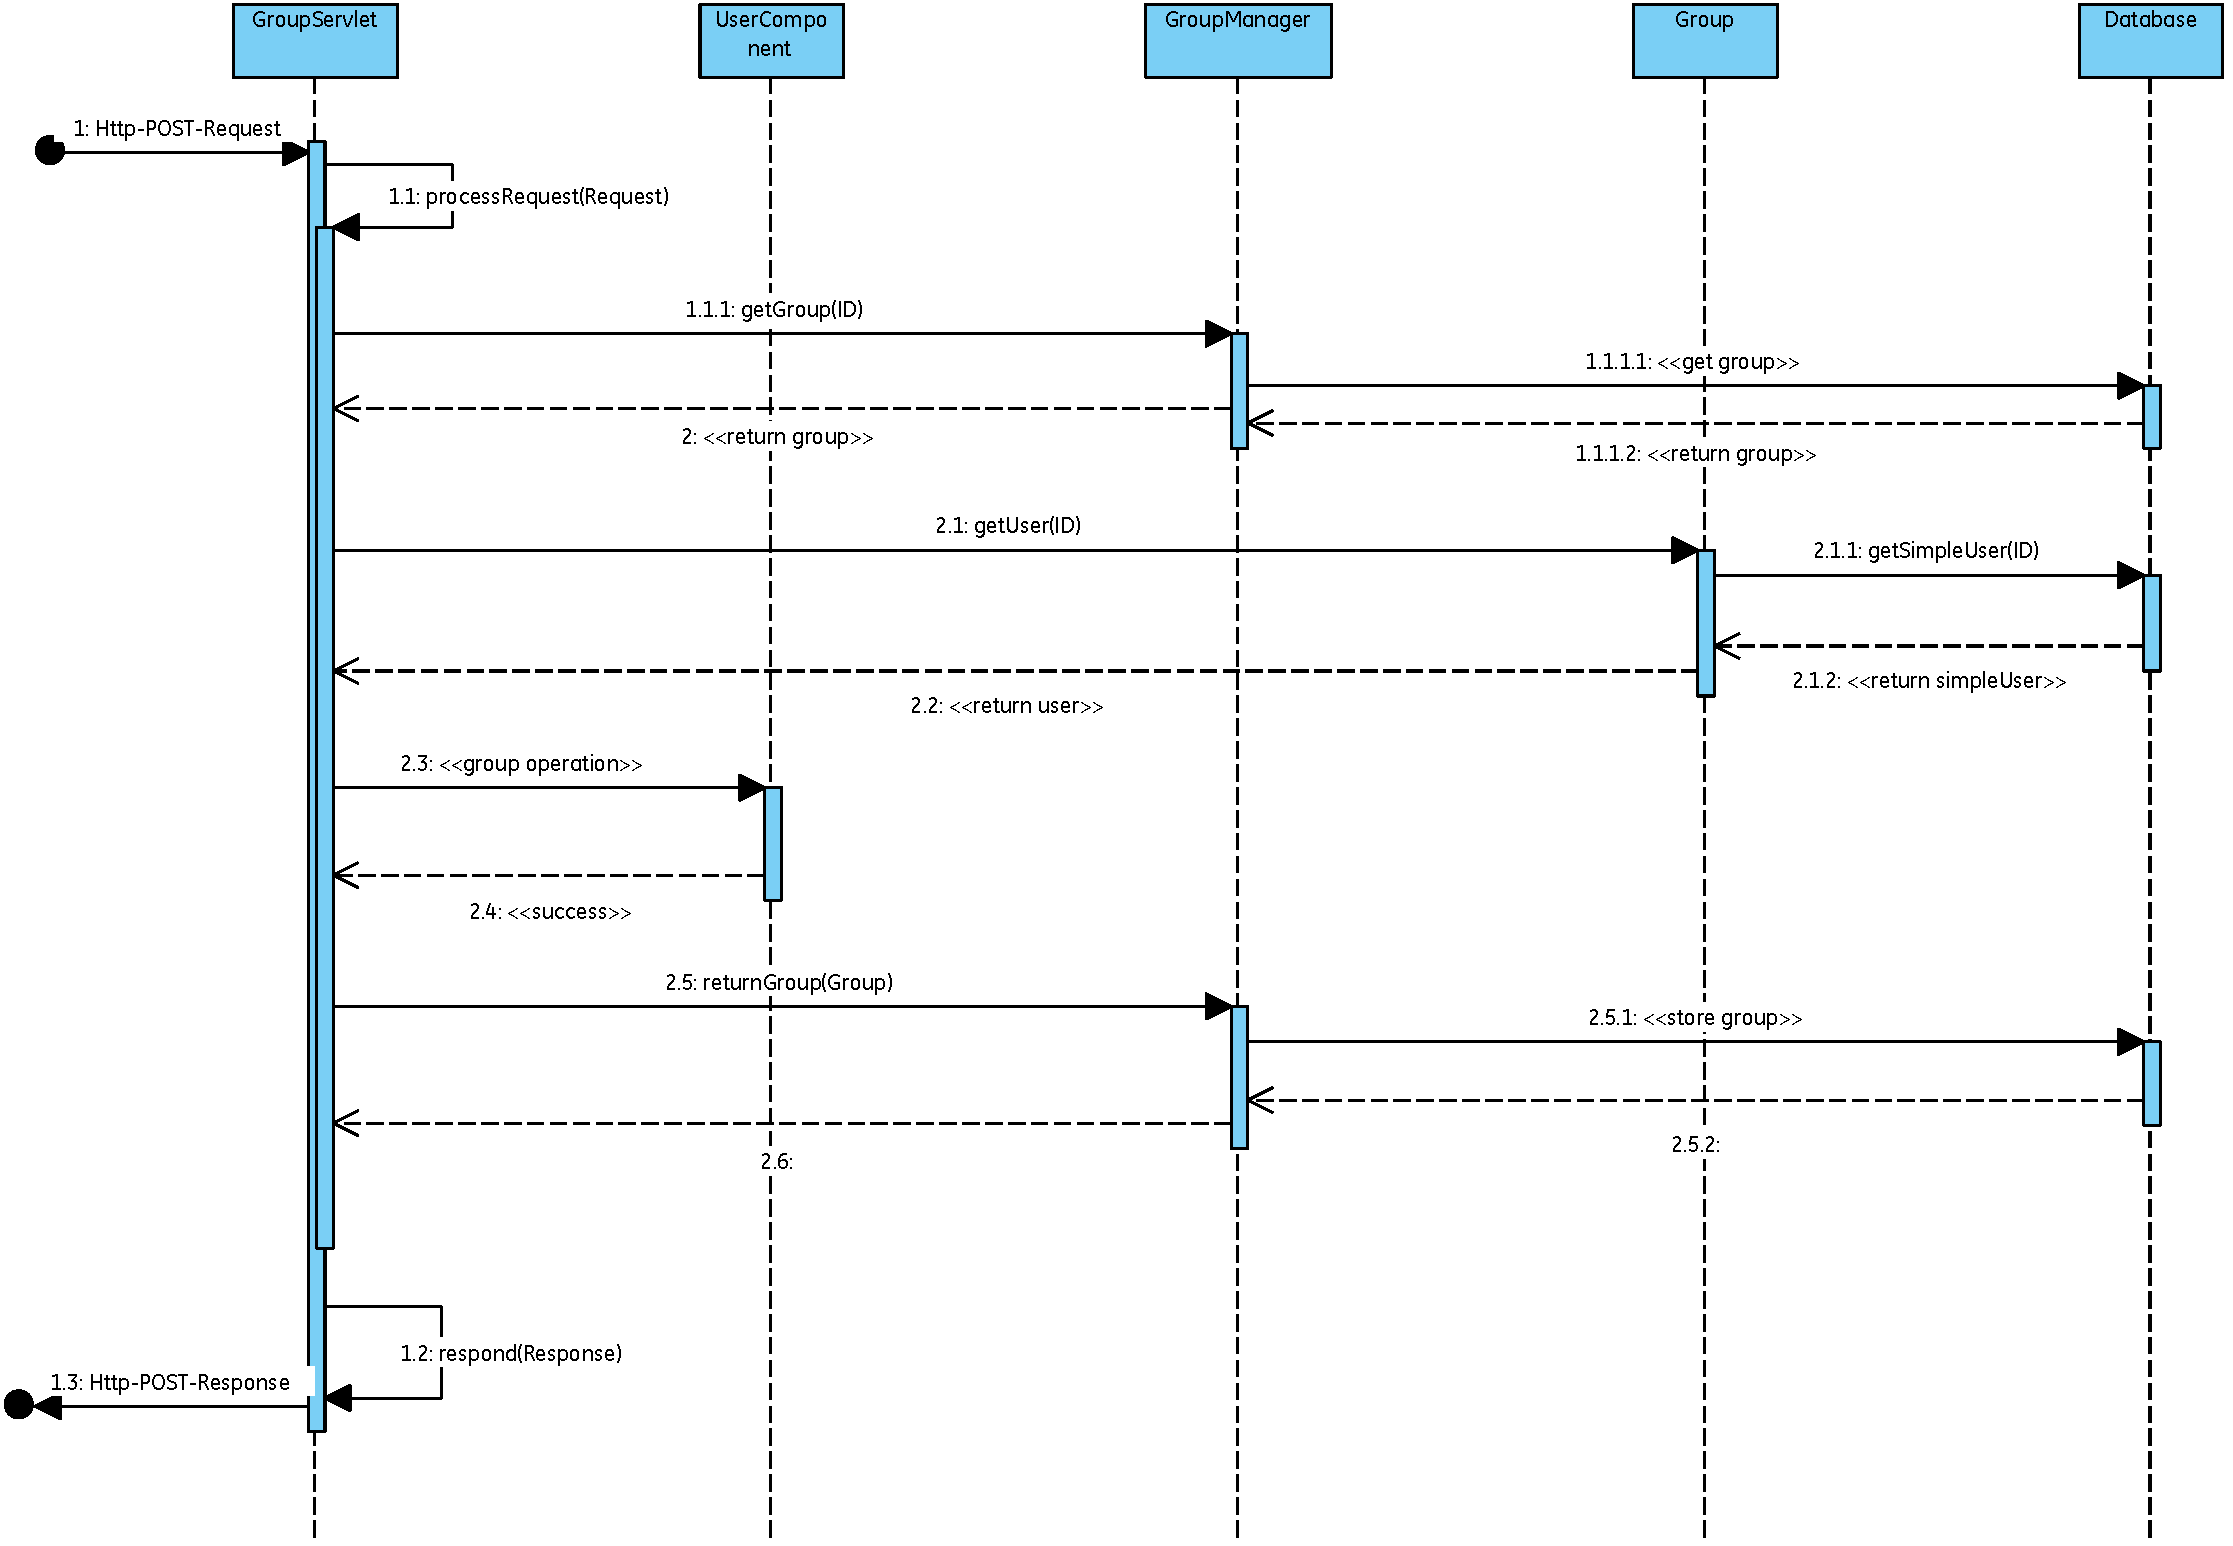
\includegraphics[scale=0.5, trim=2 2 2 2, clip=true]{servergraphs/sequenz-server.pdf}
     \caption{Sequenzdiagramm GroupServlet}
\end{figure}
\clearpage

\begin{figure}[h]
     \centering
     \hspace*{-2.9cm}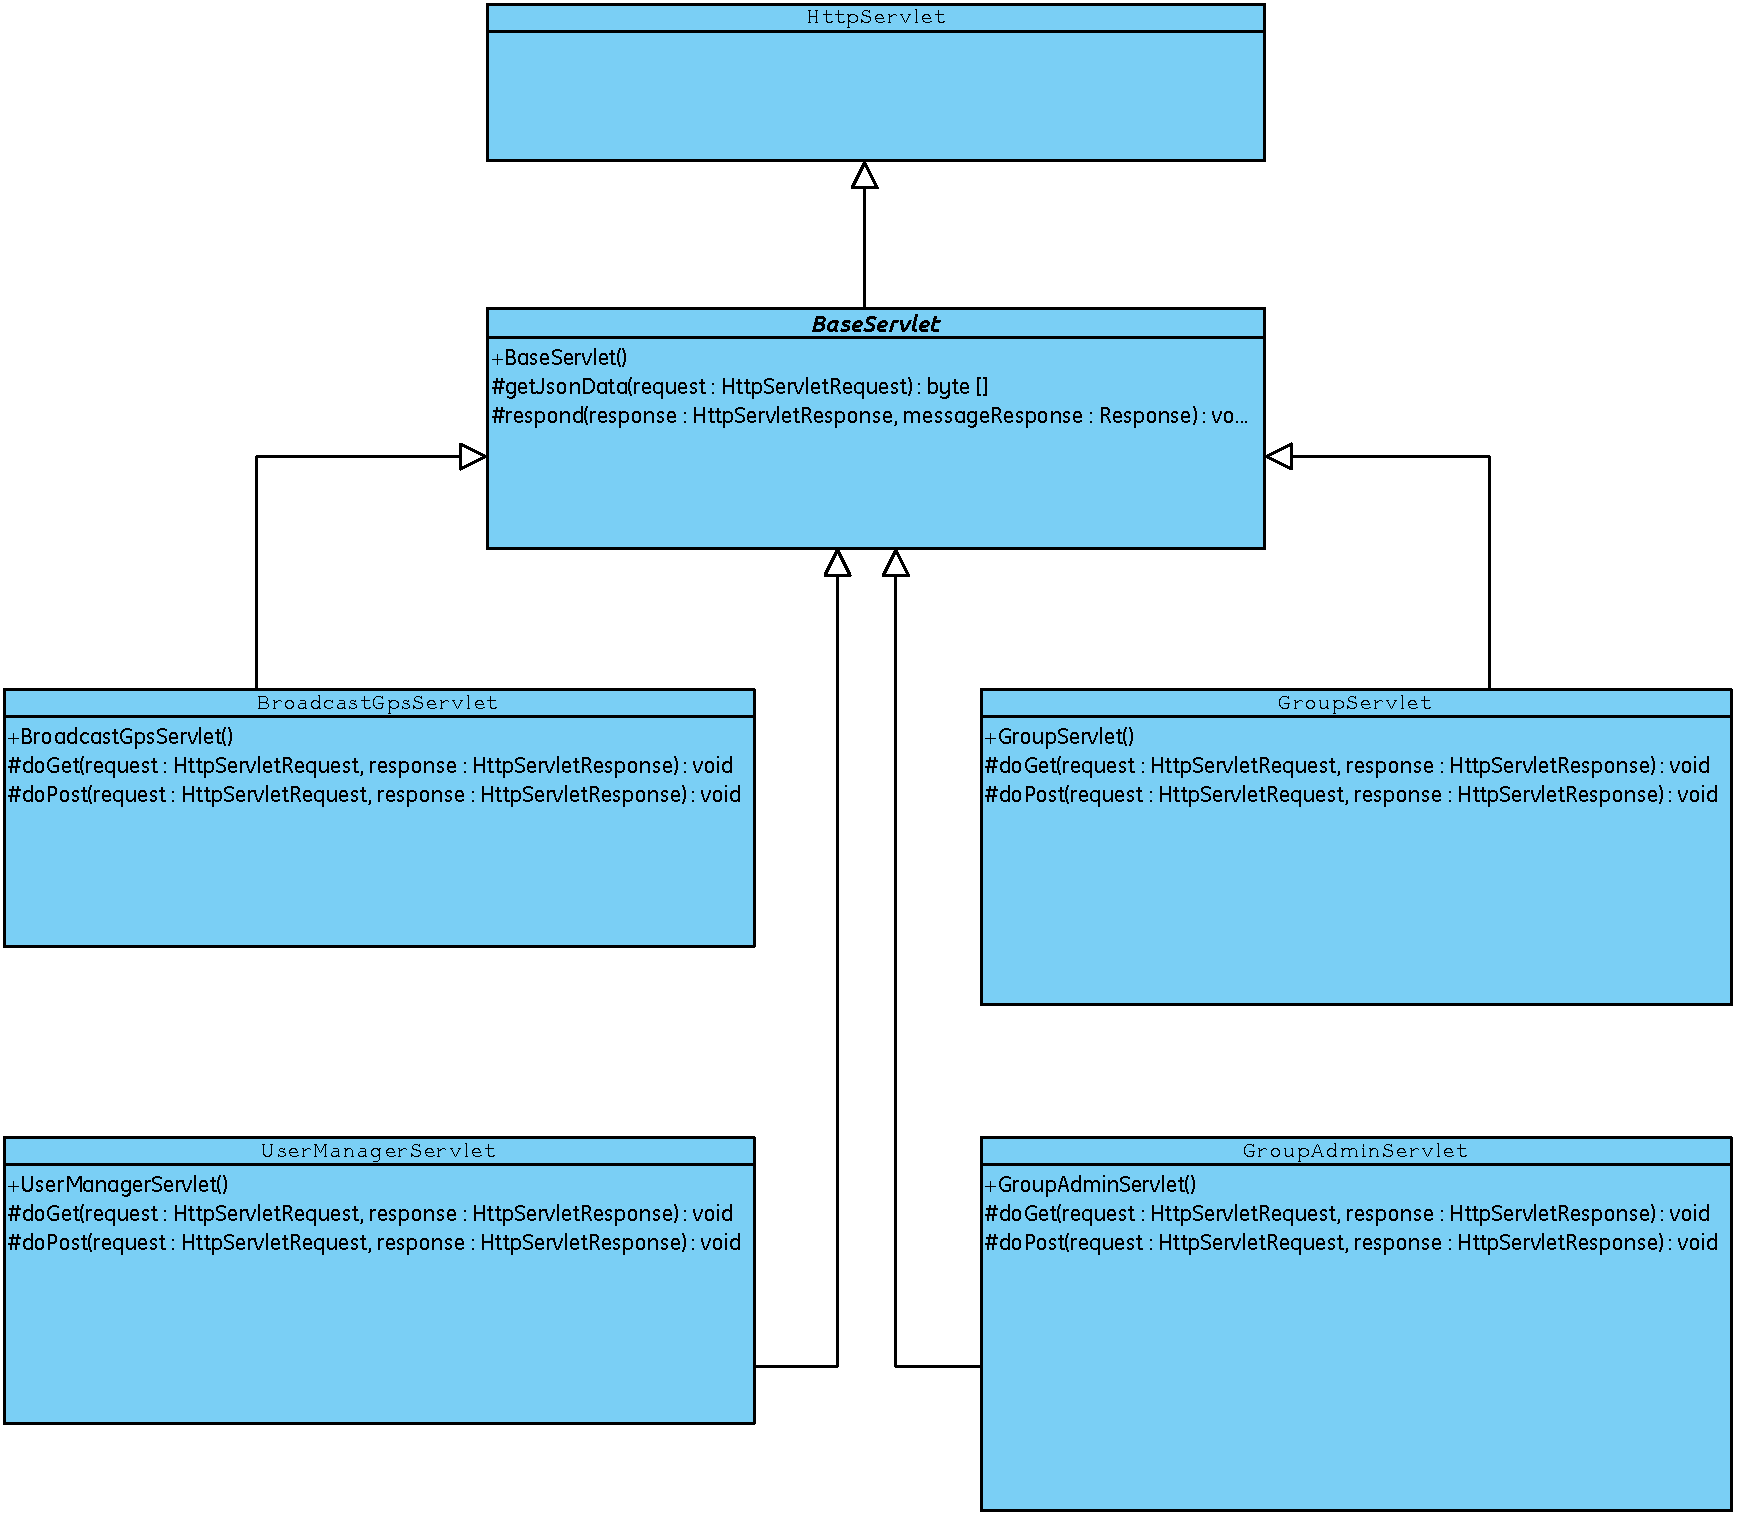
\includegraphics[scale=0.7]{servergraphs/servlets.pdf}
     \caption{Vererbungshierarchie der Servlets}
\end{figure}
\clearpage
\newpage
\textbf{Klasse GroupServlet} \\
\\
Zuständig für alle Nutzer-Anfragen bezüglich Gruppen. \\
Hier werden nur Parameter der Gruppe abgefragt. Administrative Anfragen werden vom GroupAdminServlet bearbeitet.\\
Von einem Gruppenmitglied abgefragt, werden beispielsweise aktueller Treffpunkt,\\
aktuelle Gruppenmitglieder oder aktueller Gruppenname.\\
Die GroupServlet Klasse dient als eine Schnittstelle zu der Datenbank auf dem Server.\\
Bildet die Anfrage auf ein GroupRequest Objekt ab.

\textbf{Klasse UserManagerServlet} \\
\\
Das UserManagerServlet ist für alle Benutzeroperationen zuständig. Dazu gehören:\\
Benutzeraccount anlegen, Benutzername ändern, Benutzer löschen.\\
Damit ist das UserManagerServlet eine weitere Schnittstelle zur Datenbank.\\
Bildet die Anfrage auf ein UserRequest Objekt ab.

\textbf{Klasse GroupAdminServlet} \\
\\
Im GroupAdminServlet werden alle Anfragen eines Gruppen-Administrators bearbeitet.\\
Dabei wird die Zielgruppe und der Nutzer in einem Request-Objekt übergeben.\\
Geprüft wird, ob der Benutzer Admin der Zielgruppe ist. Ist dies der Fall, \\
wird über den QueryString die gewünschte Operation auf der Gruppe ausgeführt.\\
Bildet die Anfrage auf ein GroupAdminRequest Objekt ab.

\textbf{Klasse BroadcastGpsServlet} \\
\\
In diesem Servlet werden von Gruppenmitgliedern gesendete GPS-Daten empfangen und in der
Datenbank gespeichert. Ist der GoStatus für ein Mitglied gesetzt,\\
können andere Mitglieder ihn Abrufen.\\
Bildet die Anfrage auf ein BroadcastGpsRequest Objekt ab.

\newpage
\subsubsection{Kommunikation}
Zum Datenaustausch zwischen Client und Server haben wir zwei Klassen erstellt:\\
Request und Response.\\
Davon erben die jeweils aufgabenspezifischen Request/Response-Klassen.\\
\\
\textbf{Klasse Request}\\
\\
Die abstrakte Request Klasse besteht hauptsächlich aus gettern und settern,\\
diese werden unter anderem von der Jackson API zum Serialisieren benötigt.\\
Dabei dient die Klasse ausschließlich als container und enthält keine Programmlogik.\\
Wichtig ist, dass nur ID's bzw. Namen in Form von String/Integer übergeben werden,\\
dadurch wird die Größe des resultierenden JSON-Strings möglichst klein gehalten.\\
\\ \\ \\

\begin{figure}[h]
     \centering
     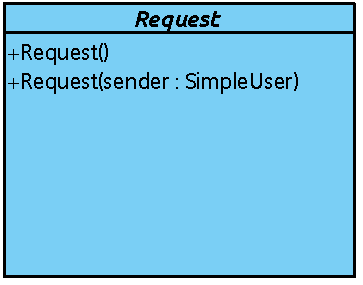
\includegraphics[scale=1.0,trim=2 2 2 2,clip=true]{servergraphs/request.pdf}
     \caption{Klassendiagramm Request}
\end{figure}
\clearpage

\begin{figure}[h]
\hspace*{-1.8cm}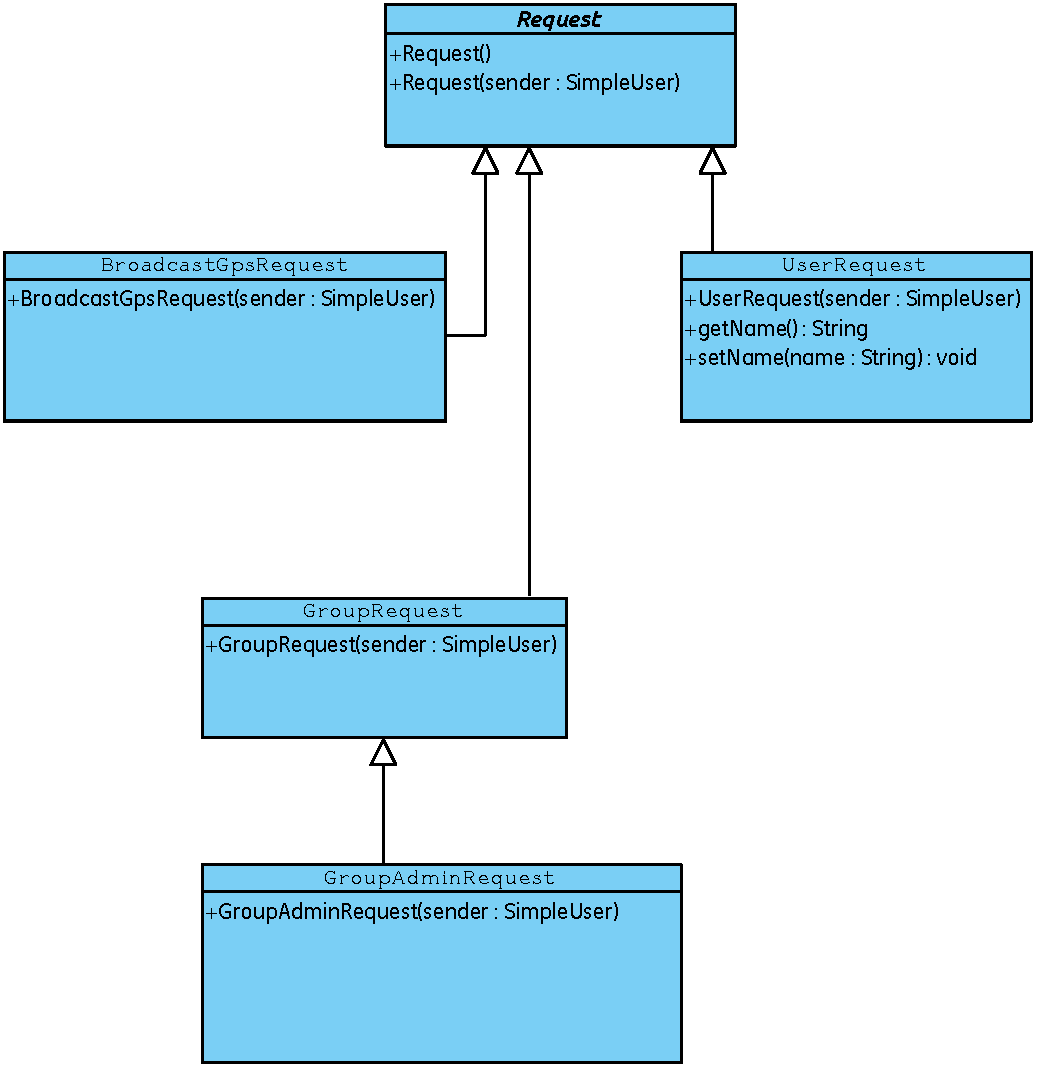
\includegraphics[scale=1.0,trim=2 2 2 2,clip=true]{servergraphs/communication-request.pdf}
     \caption{Vererbungshierarchie Request}
\end{figure}
\clearpage

\textbf{Klasse UserRequest}\\
\\
UserRequest ist eine Anfrage um einen neuen Benutzeraccount anzulegen, \\
bzw. falls schon vorhanden, den Benutzernamen zu ändern.\\

\textbf{Klasse GroupRequest}\\
\\
Alle gruppenbezogenen Anfragen. Benötigt werden Benutzer-ID, Name der entsprechenden
Gruppe, und ein QueryString, der die Operation beschreibt, die auf der Gruppe\\
ausgeführt werden soll.\\
Dieser Anfragetyp kann nur von einem Gruppenmitglied gesendet werden.\\
Diese Anfrage kann gesendet werden um den aktuellen Stand einer Gruppe abzufragen.\\
Änderungen sind zum Beispiel wenn ein neuer Treffpunkt gesetzt wurde, \\
ein Benutzer der Gruppe beigetreten ist, oder ein Benutzer die Gruppe verlassen hat.\\

\textbf{Klasse GroupAdminRequest}\\
\\
GroupAdminRequest ist eine erweiterung der normalen GroupRequest. Sie enthält\\
zusätzlich alle Anfragen eines Gruppenadministrators. Dazu zählen: Gruppe löschen,\\
Gruppe umbenennen, Mitglieder einladen, etc.\\
Die Klasse hält die Variablen für jede mögliche Administrator-Anfrage.\\

\textbf{Klasse BroadcastGpsRequest}\\
\\
Anfrage um die eigenen GPS-Daten an die Gruppe zu verteilen, oder GPS-Daten der\\
anderen Gruppenmitglieder abzufragen.\\
Die eigenen GPS-Daten sind nicht zwingend notwendig, da das anfragende Mitglied seinen\\
Status auf 'Go' setzen kann, ohne die eigenen GPS-Daten preiszugeben.\\

\newpage
\textbf{Klasse Response}\\
\\
Als Antwort auf eine Request sendet der Server eine Response an den Client.\\
Die Response enthält alle angeforderten Daten bzw. manipulierte Daten und \\
ob die Operation, die der Nutzer angefragt hat, erfolgreich war.\\
Auf einfache Anfragen, wie beispielsweise den eigenen Benutzernamen zu ändern,\\
wird mit einer einfachen Response geantwortet, die dem Nutzer sagt,\\
ob der Name erfolgreich geändert wurde.\\
\\ \\ \\ \\

\begin{figure}[h]
     \hspace*{-2cm}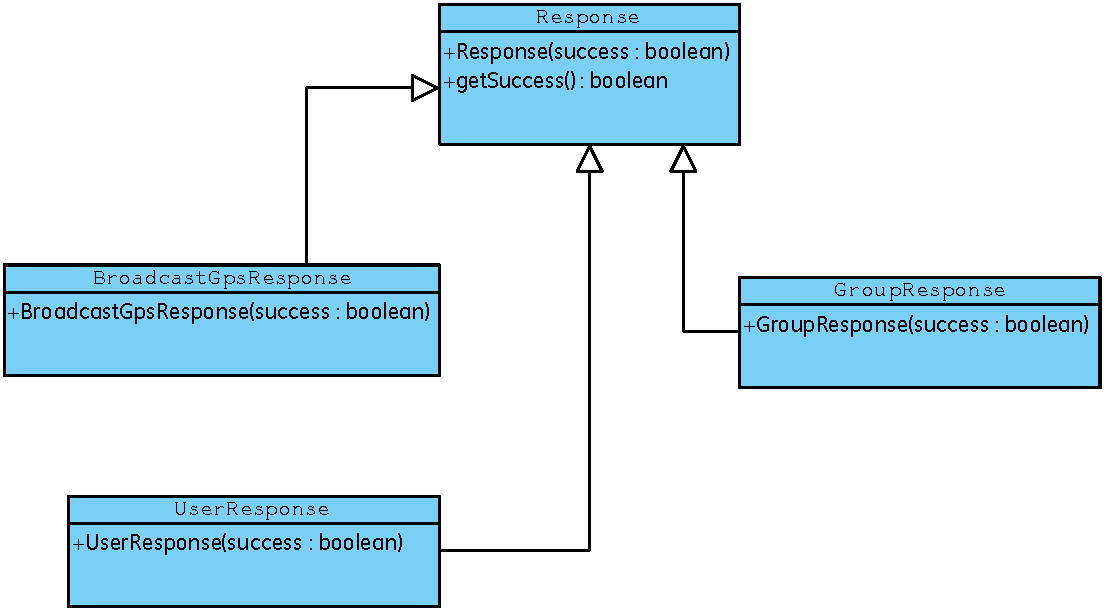
\includegraphics[scale=1.0]{servergraphs/communication-response.pdf}
     \caption{Vererbungshierarchie Response}
\end{figure}
\clearpage

\textbf{Klasse UserResponse}\\
\\
Anwort auf eine Nutzername ändern Anfrage oder eine Registrieren Anfrage.\\
Bei der Registrierung wird eine eindeutige Benutzer-ID zurückgegeben.\\
Im Falle einer Benutzername-ändern-Anfrage wird nur der Status zurückgegeben.\\

\textbf{Klasse GroupResponse}\\
\\
Antwort auf eine Gruppen-Anfrage oder eine Administrator-Anfrage.\\
Ein GroupResponse-Objekt enthält dabei die, nach der Operation, aktuelle Gruppe.\\
Bei einer Update-Anfrage wird ebenfalls mir einer GroupResponse geantwortet.\\

\textbf{Klasse BroadcastGpsResponse}\\
\\
Als Antwort auf eine BroadcastGpsRequest, enthält die BroadcastGpsResponse die GPS-Daten\\
der anderen Gruppenmitglieder, die bereits 'Go' gedrückt haben, also ihre Daten bereits\\
an den Server gesendet haben.\\
\newpage

\subsubsection{Server-Modell}
Das Modell des Servers unterscheidet sich in wesentlichen Punkten zu dem des Clients:\\
Operationen auf Gruppen oder Benutzern lösen keine Anfragen an einen Server aus,\\
sondern arbeiten direkt mit der Schnittstelle zur Datenbank.\\
Das Client-Modell stellt praktisch die 'Fernbedienung' für das Server-Modell dar.\\
\\
\textbf{Hibernate}\\
\\
Die Schnittstelle unserer Datenbank stellt Hibernate dar. Dazu werden in den Klassen
GroupAdminServer, GroupMemberServer und SimpleUser (Also alles was gespeichert werden muss), Annotations gesetzt, die Hibernate zum Abbilden benötigt.
Anfragen an die Datenbank werden von GroupManager und UserManager gesteuert.\\
\\
\textbf{Klasse UserManager}\\
\\
Der UserManager verwaltet Benutzeraccounts und bietet eine allgemeine Schnittstelle\\
zur Datenbank. Er hat zwei Methoden um ein Benutzer-Objekt aus der Datenbank\\
anzufordern: getUserById(int ID) - durchsucht die Datenbank nach einem User mit\\
gegebener Nutzer-ID und getUserByDevId(String devID) - durchsucht die Datenbank\\
nach einem Benutzer mit passender Geräte-ID. \\
Darüber werden die meisten Benutzer identifiziert, die eine Anfrage senden.\\
Die Nutzer-ID ist dazu gedacht, dass Gruppenmitglieder nicht die Geräte-ID der \\
anderen Mitglieder erfahren.\\
createUser(String Name) - Erzeugt einen Neuen Benutzer mit gegebenem Namen.\\
deleteUser(String devId) - Löscht den Benutzer mit der gegebenen Geräte-ID.\\
\\ \\ \\

\begin{figure}[h]
     \centering
     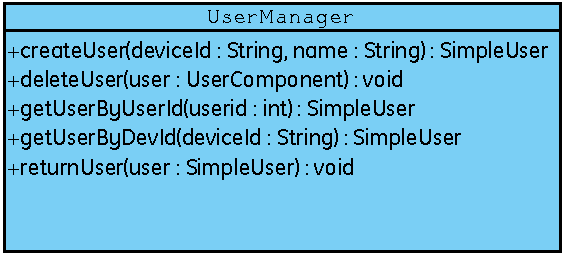
\includegraphics[scale=1.0, trim=1 1 1 1,clip=true]{servergraphs/user-manager.pdf}
     \caption{Klassendiagramm UserManager}
\end{figure}
\clearpage

\textbf{Klasse GroupManager}\\
\\
Gleichermaßen wir der UserManager, bietet auch der GroupManager eine \\
Schnittstelle zur Datenbank. Er bietet die Fabrikmethode createGroup()\\
zum Erstellen neuer Gruppen. Die Methode legt dazu einen neuen Eintrag in der\\
Datenbank an und liefert das neue Group-Objekt zurück.\\



\begin{figure}[h]
     \centering
     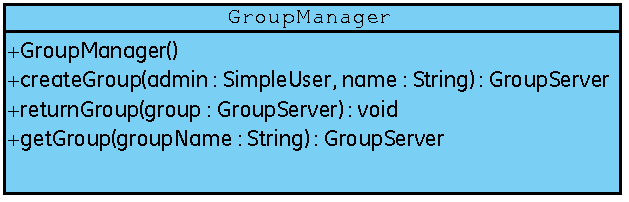
\includegraphics[scale=1.0, trim=2 2 2 2, clip=true]{servergraphs/group-manager.pdf}
     \caption{Klassendiagramm GroupManager}
\end{figure}
\clearpage

\textbf{Klasse GroupServer}\\
\\
Serverseitige Darstellung einer Gruppe. Operationen werden auf der Gruppe nicht\\
direkt ausgeführt. Nach dem Erstellen der Gruppe, laufen alle Operationen über den\\
Gruppenadministrator. über getMember(ID) bekommt man das Mitglied, dass man in \\
der aktuellen Gruppe darstellt. Also entweder GroupMember oder GroupAdmin.
In der Fabrikmethode getMember(ID) wird dem UserDecoratorServer das Gruppen-Objekt\\
übergeben, an dass dieser dann gebunden ist.\\


\begin{figure}[h]
     \centering
     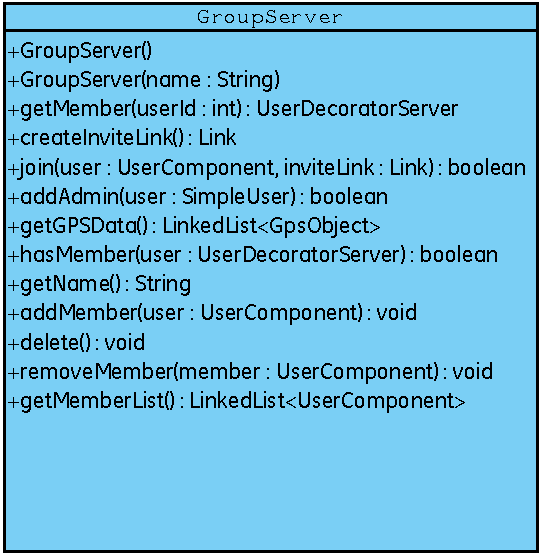
\includegraphics[scale=1.0, trim=2 2 2 2, clip=true]{servergraphs/group-server.pdf}
     \caption{Klassendiagramm GroupServer}
\end{figure}
\clearpage

\textbf{Klasse LinkGenerator}\\
\\
Die Aufgabe des LinkGenerators besteht darin, zu einer gegebenen Gruppe einen \\
Einladungslink zu generieren. Dabei wird an die Basis-URL des GroupServlets der\\
Gruppenname und ein zufällig generierter String angehängt.\\


\begin{figure}[h]
     \centering
     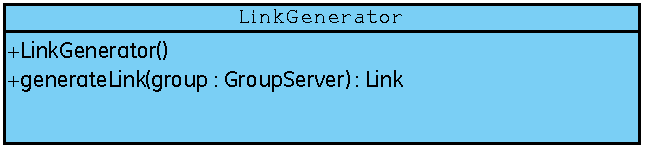
\includegraphics[scale=1.0, trim=2 2 2 2, clip=true]{servergraphs/link-generator.pdf}
     \caption{Klassendiagramm LinkGenerator}
\end{figure}
\clearpage

\textbf{Klasse Link}\\
\\
Da die Klasse Link aus dem common package für Client bereits dokumentiert ist,\\
sind hier nur noch ein paar Anmerkungen.
Ein Link vom Administrator einer Gruppe erzeugt und ist an die Gruppe gebunden.\\
Diese Klasse repräsentiert eine Gruppeneinladung. über die Getter kann man unabhängig\\
den Gruppennamen und das Geheimnis abfragen.\\
Hat man als Administrator den Link vom Server erhalten, wird über die toString() \\
Methode die endgültige URL erstellt. Diese kann nun über andere Wege versendet werden.
Öffnet man eine zugesendete URL mit der GoApp, wird daraus eine GroupRequest erzeugt,
mit der ein anderer Nutzer der Gruppe beitreten kann.\\
Das Geheimnis wird im zugehörigen Gruppen-Objekt gespeichert.\\
\\ \\ \\
\begin{figure}[h]
     \centering
     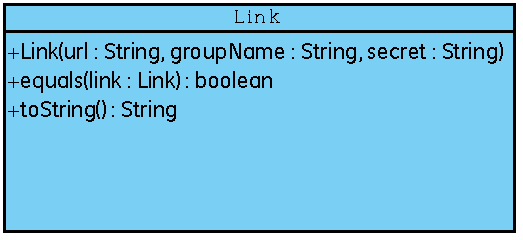
\includegraphics[scale=1.0, trim=2 2 2 2, clip=true]{servergraphs/link.pdf}
     \caption{Klassendiagramm LinkGenerator}
\end{figure}
\clearpage

\newpage
\textbf{Klasse UserDecoratorServer}\\
\\
Das serverseitige Gegenstück zum UserDecorator. Er implementiert das gleiche Interface
wie der UserDecorator auf dem Client, nur dass er mit GroupServer arbeitet. \\
Im UserDecoratorServer sind sowohl die Methoden des Admins, wie auch die des\\
einfachen GroupMembers vorhanden. Die Idee dahinter ist, dass man nicht verhindern\\
kann, dass ein normaler GroupMember eine Admin-Anfrage sendet.\\
Die Implementierung der beiden Klassen unterscheidet dann das Verhalten.\\
(Siehe GroupAdminServer und GroupMemberServer)\\



\begin{figure}[h]
     \centering
     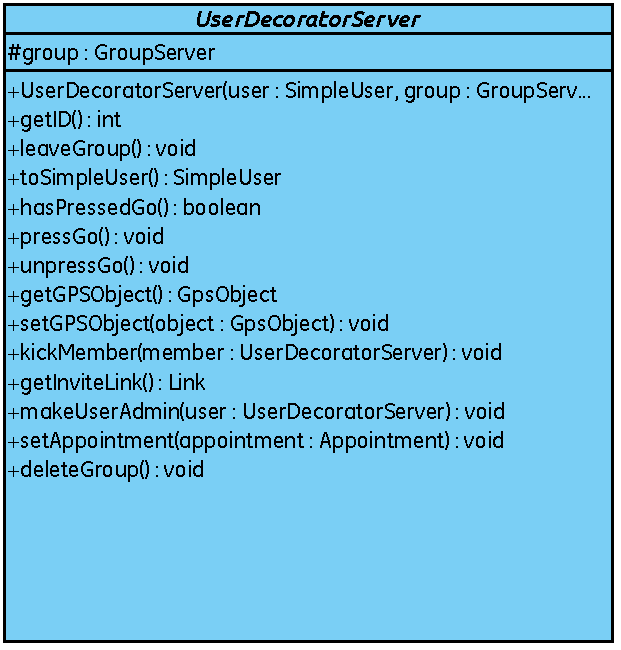
\includegraphics[scale=0.9]{servergraphs/user-decorator-server.pdf}
     \caption{Klassendiagramm UserDecoratorServer}
\end{figure}
\clearpage

\begin{figure}[h]
     \centering
     \hspace*{-2.6cm}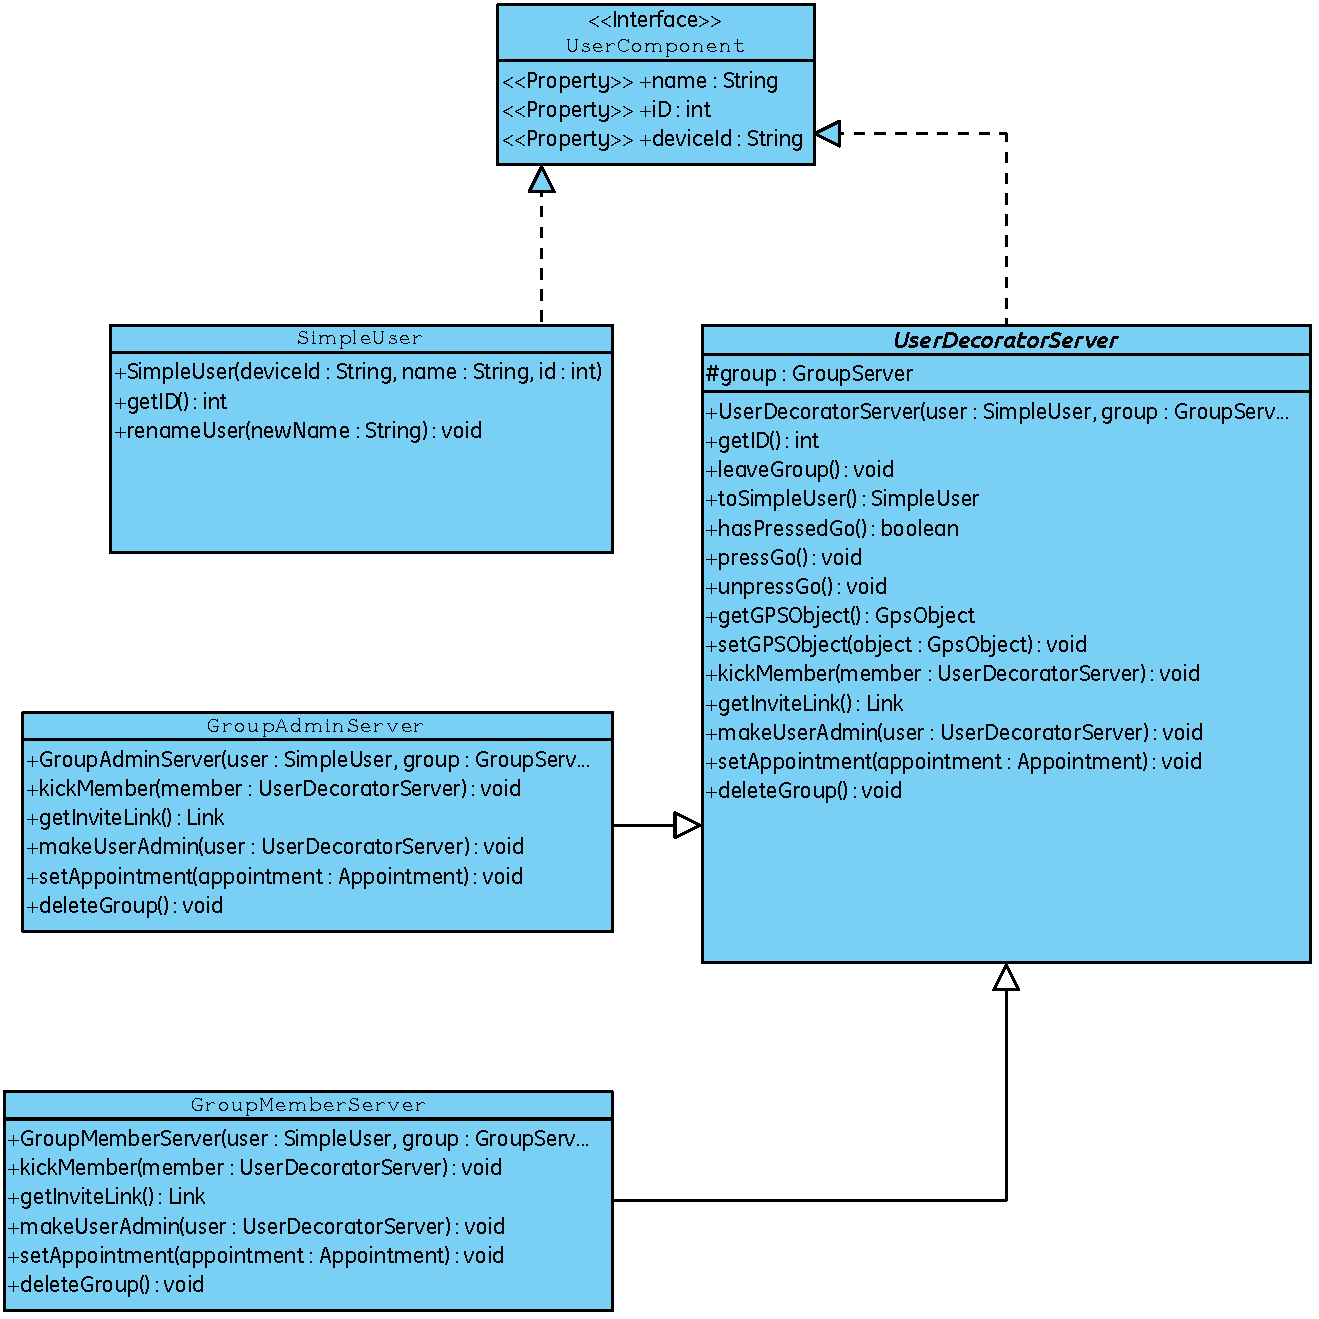
\includegraphics[scale=0.9]{servergraphs/user-component.pdf}
     \caption{Klassenhierarchie UserDecoratorServer}
\end{figure}
\clearpage

\textbf{Klasse GroupMemberServer}\\
\\
Die serverseitige Klasse für Gruppenmitglieder. Die einfache Implementierung eines\\
Gruppenmitglieds ohne besondere Rechte.\\
Die Klasse GroupMemberServer implementiert auch die Methoden des Administrators,\\
falls ein skrupelloses Gruppenmitglied eine Admin-Anfrage sendet, wird dabei\\
jedoch eine Fehlermeldung ausgelöst.\\

\textbf{Klasse GroupAdminServer}\\
\\
Die Gruppen-Administrator Klasse auf dem Server steuert alle Gruppenoperationen,\\
das heißt, wenn man über group.getUser(ID) ein Objekt der Klasse GroupAdminServer\\
zurückbekommt, kann man darüber die Gruppe 'group' kontrollieren.\\
Als Indirektion ruft der
Die Operationen sind an die Gruppe gebunden, auf der man getUser(ID) aufruft.\\

